\documentclass[11pt, oneside]{article}

% Import Packages
\usepackage{amsmath}
\usepackage{amssymb}
\usepackage{comment}
\usepackage{cancel}
\usepackage{hyperref}

% Page setup
\usepackage[
legalpaper, 
top=1in, 
bottom=1in, 
left=1.5in, 
right=1.5in
]{geometry}

% Import graphicx and set figure path
\usepackage{graphicx}
\graphicspath{ {./img/} }

% Define SIUnit Commands
\usepackage{siunitx}
\newcommand{\h}{\unit{\hour}}
\newcommand{\ph}{\unit{\per\hour}}
\newcommand{\um}{\unit{\micro\metre}}
\newcommand{\pums}{\unit{\per\micro\metre\squared}}
\newcommand{\nm}{\unit{\nano\mole\per\litre}}

% Add Bibliography
\usepackage[
backend=biber,
style=apa,
sorting=ynt
]{biblatex}
\addbibresource{sources.bib}

% Create supplementary figure environment
\usepackage{caption}
\usepackage{newfloat}
\DeclareFloatingEnvironment{supplementaryfigure}
\captionsetup[supplementaryfigure]{name=Supplementary Figure}

\emergencystretch=1em

\begin{document}

\title{Brassinosteroid and CLASP-driven Models of Root Zonation in \emph{A. Thaliana}}
\author{Riley Wheadon, Geoffrey Wasteneys, Eric Cytrynbaum \\ University of British Columbia}
\date{September 8th, 2024}
\maketitle

\section{Abstract}

The CLASP protein has been shown to influence cell growth by changing the arrangement of cellulose microfibrils via the orientation of microtubule arrays (MTs) on the cell membrane.
Here we present a mathematical model of this phenomenon which we verify against \emph{in vivo} observations of \emph{A. thaliana} roots. 
Our model uses data from the brassinosteroid (BR) signalling pathway and predicts its downstream effects on CLASP, MTs, and ultimately root growth. 
Additionally, the model accurately explains the behaviour of various mutant roots in which elements of the aforementioned signalling network are edited or removed. 
We find that BR signalling alone is unable to predict observed rates of cell growth in the root and conclude that CLASP is essential for root zonation.



\newpage

\section{Introduction}

\subsection{Root Zonation}

The growing root of \emph{A. thaliana} can be roughly divided into six distinct zones, with the cells in each zone exhibiting qualitatively distinct behaviour. At the tip of the root lies the root cap, a region of cells that are constantly sluffed off to protect the growing root from debris (\cite{kumpf2015}). Above the root cap is a small group of static cells known as the quiescent centre (henceforth QC), which play a crucial role in the regeneration of the root cap and surrounding cells (\cite{matosevich2021}). The models presented in this paper will ignore these two regions and measure position within the root as the distance in $\um$ from the QC. 

\medskip

In the meristematic zone (henceforth MZ), cells experience rapid cell division and slower cell growth. In this region, cells grow from $4.5\um$ to $9\um$ over a period of about $18\h$ (\cite{verbelen2006}) while moving from $0\um$ to $200\um$ above the QC. Above the meristematic zone is the transition zone (henceforth TZ), in which cells experience lower rates of division and grow from $9\um$ to $30\um$ over the course of $10\h$ (\cite{verbelen2006}). The TZ spans from approximately $200\um$ to $520\um$ above the QC. Next to the TZ is the elongation zone (henceforth EZ), where cells grow rapidly from $30\um$ to $130\um$ over the course of $4\h$ (\cite{verbelen2006}). After leaving the EZ at approximately $900\um$ above the QC, cells begin differentiation and cease growth. Thus the final and most proximal region of the root is aptly named the differentiation zone (henceforth DZ).

\subsection{CLASP and Microtubules}

Microtubules (henceforth MTs) are tubulin polymers located on the plasma membrane of the cell which guide the deposition of cellulose on the cell wall (\cite{hamant2010}). When the MTs and cellulose microfibrils are deposited orthogonally to the axis of growth, the cell experiences anisotropic growth. If the MTs and cellulose are less organized, then the turgor pressure within the cell faces isotropic resistance which ultimately inhibits growth (\cite{hamant2010}).

\medskip

The CLASP protein plays an essential role in MT patterning through its ability to help MTs cross sharp edges on the cell membrane (\cite{ambrose2011}). 
This results formation of bundles of MTs along the transverse, radial, and longitudinal edges of the cell (\cite{halat2022}). 
Bundles along the transverse and radial edges (henceforth TFBs), are of particular interest because they lead to microtubule arrangements that run parallel to the axis of growth.
These TFBs disrupt the formation of circumferential cellulose microfibrils, which ultimately inhibits cell growth (\cite{halat2022}).

\medskip

Cell length modulates the effect of CLASP on MT patterning due to the fact that longer cells have longer longitudinal edges relative to their radial and transverse edges. This causes the CLASP protein to localize towards the longitudinal edges and away from the radial and transverse edges, leading to a reduction in TFBs and an increase in growth (\cite{halat2022}). A diagram of this phenomenon from \cite{halat2022} is shown in Figure \ref{fig:clasp-length-effect}.

\begin{figure}
    \centering
    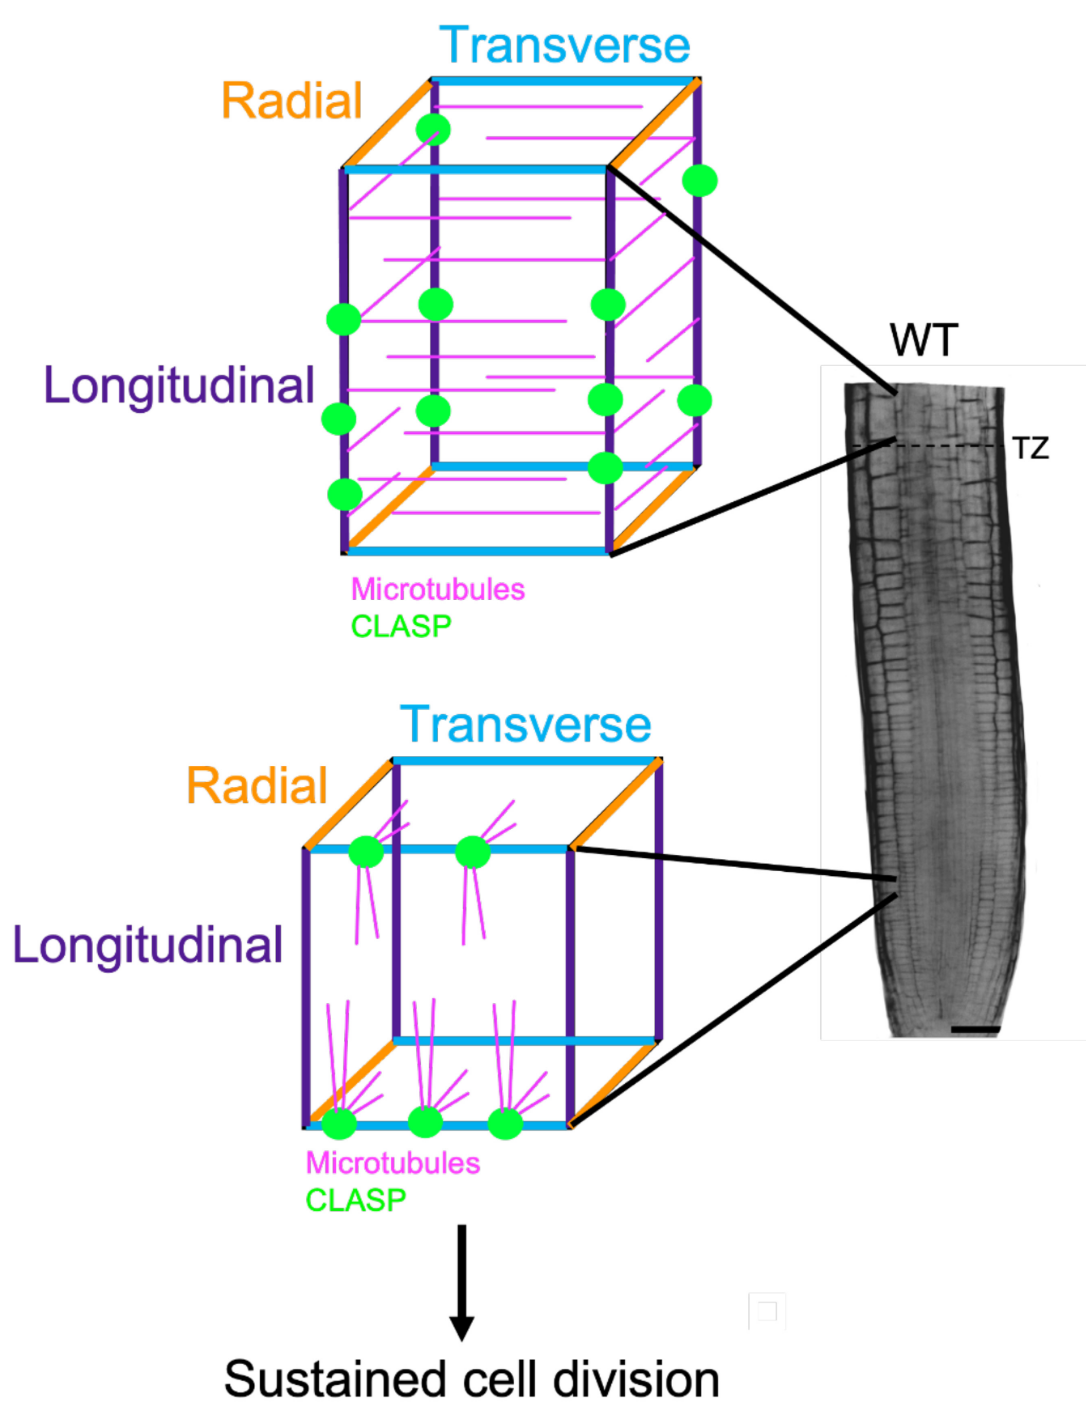
\includegraphics[width=8cm]{img/clasp-length-effect.png}
    \caption{In longer cells, CLASP localizes to the longitudinal edges which drives a reduction in TFBs and promotes cell growth.}
    \label{fig:clasp-length-effect}
\end{figure}


\subsection{Brassinosteroid}

Brassinosteroids (BRs) are a class of plant hormones that have shown to promote both longitudinal and radial growth in a spatiotemporal manner (\cite{ackerman-lavert2020}). Extracellular BRs, particularly brassinoslide (henceforth BL), bind to the BR receptor BRI1 and its homologues on the cell membrane (\cite{vukasinovic2021}). This releases the inhibition of the BZR1/BES1 transcription factors by the BIN2 signalling inhibitor (\cite{ackerman-lavert2020}). The effects of BR signalling have been shown to be stronger in the TZ and stronger still in the EZ due to a higher concentration of BR precursors (\cite{vukasinovic2021}). 

\medskip

The BZR1/BES1 transcription factors, which are often used as a proxy for BR signalling, have been shown to inhibit CLASP by binding directly to its promoter and repressing its activity (\cite{ruan2018}). Additionally, CLASP influences the BR signalling network by promoting the recycling of endocytosed BRI1 receptors. Together, these two effects produce a stable postive-negative feedback loop that helps to ensure homeostasis in the root (\cite{ruan2018}).

\subsection{Mutant Roots}

Making small changes to the network of proteins and hormones described in the prior two sections leads to significant changes in root phenotypes. This paper explores the \emph{clasp-1} (\cite{ambrose2007}) \emph{brinCLASPpro} (\cite{ruan2018}) mutant roots. The \emph{clasp-1} root has a loss-of-function mutation that entirely inhibits the production of CLASP, which ultimately leads to an increase in cell growth through the previously discussed pathway (\cite{halat2022}). However, the rapid cell growth results in fewer cell divisions and thus fewer cells in the \emph{clasp-1} root (\cite{halat2022}), resulting in a lower rate of overall root growth relative to the wild type (\cite{ambrose2007}). 


\medskip

In wild type roots, the transcription of the CLASP protein is inhibited whenthe root is exposed to exogenous BRs (\cite{ruan2018}). However, the \emph{brinCLASPpro} root is insensitive to the effects of BR signalling, meaning the application of exogenous BRs does not affect the amount of CLASP in this mutant. It therefore stands to reason that the \emph{brinCLASPpro} mutant should have more CLASP than the wild type due to the abscence of this inhibition. It has been shown that an excess of CLASP upregulates the level of BR signalling by promoting the recycling of BRI1 receptors (\cite{ruan2018}), and we speculate that this leads to the increased cell growth observed in \emph{brinCLASPpro} mutants relative to the wild type. A plot of cell size across the mutants and the wild type is shown in Figure \ref{fig:mutant-sizes}.

\medskip

\begin{figure}[!htbp]
    \centering
    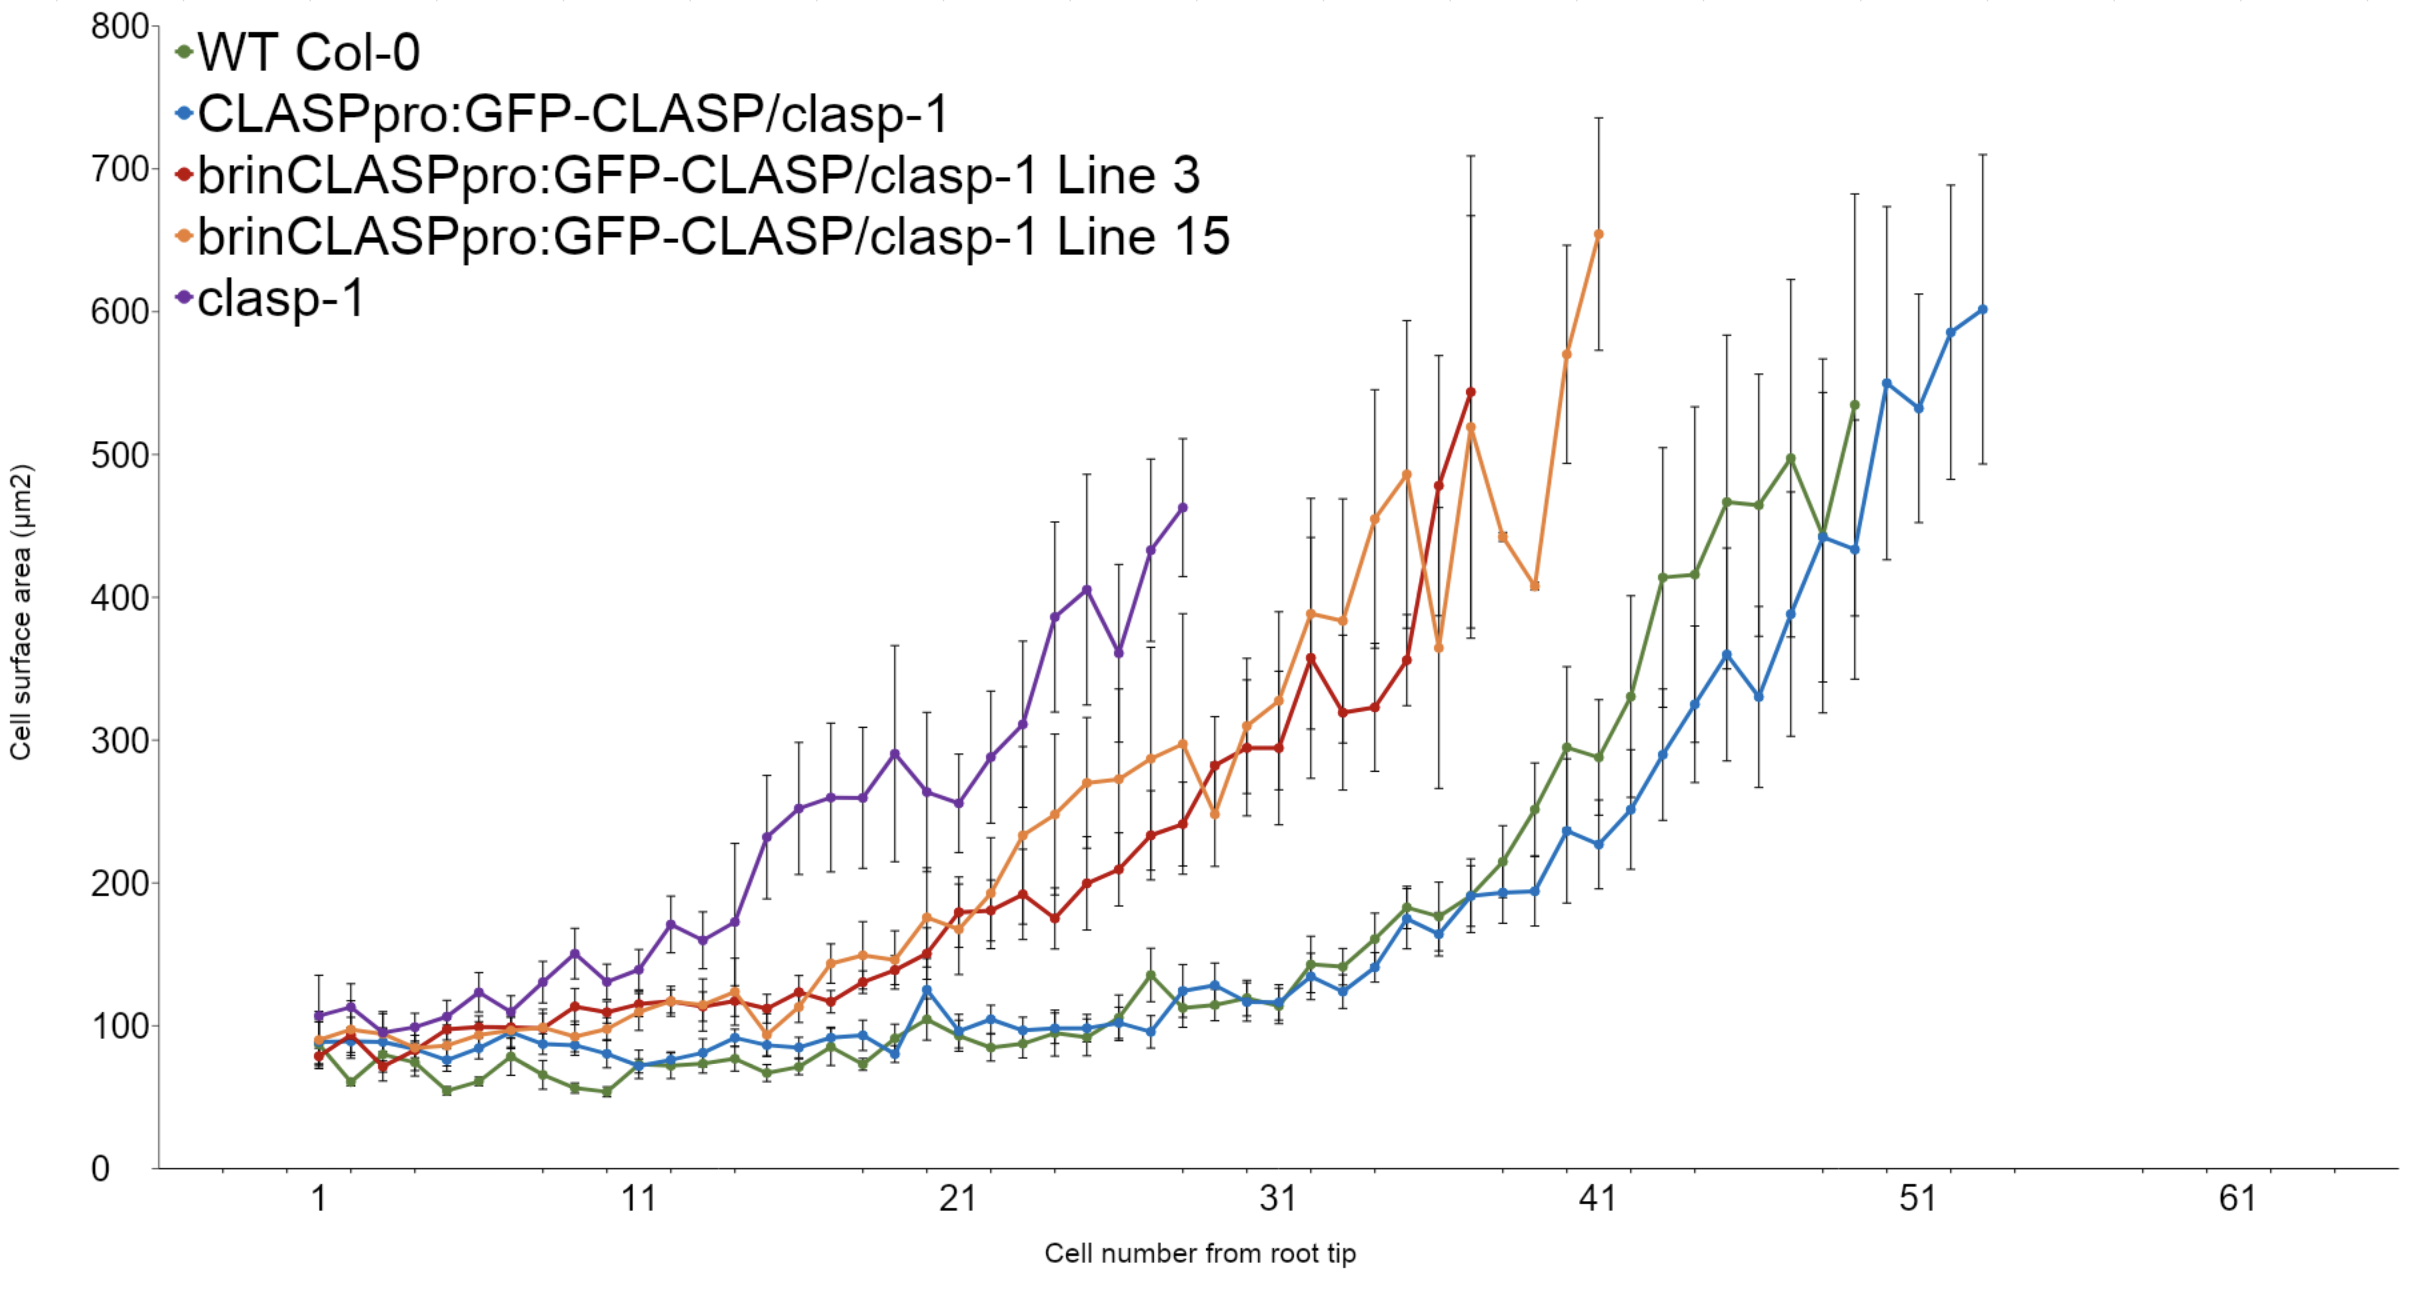
\includegraphics[width=13cm]{img/mutant-cell-sizes.png}
    \caption{Average cell areas plotted against cell number for each of the two mutant roots and the wild type. This data was taken from trichoblast cell columns in the epidermis. The GFP-CLASP line drives the expression of a fluorescent fusion protein which fully complements the \emph{clasp-1} mutant (\cite{ambrose2011}). Therefore, the GFP-CLASP/clasp-1 root is phenotypically similar to the wild type. Observe that the \emph{clasp-1} mutant has the largest cells, followed by the \emph{brinCLASPpro} mutant, followed by the wild type.}
    \label{fig:mutant-sizes}
\end{figure}









\newpage

\section{Cell Column Model}

Our first model of CLASP-driven root growth in \emph{A. thaliana} aims to qualitatively explain the phenomenon of cell zonation. A quantitative analysis of the differences in behaviour between the mutants is presented in Supplementary Figure \ref{sfig:data-trichoblast} and \ref{sfig:trichoblast-distribution}. In this model, each cell has a length $L$ which increases with time. Every cell also has a division level $D$. When $D > 1$, the cell divides into two cells with length $L / 2$ and division level $D = 0$. We model the changes in $L$ and $D$ over an arbitrary time scale using a number of assumptions described in the subsequent paragraphs.

\medskip

A cell can divide every $1/d_{0}$ time units at most. Cells must be at least $9\um$ long in order to divide (\cite{verbelen2006}). The cell division rate is inhibited by the length of the cell. By making this assumption, we treat cell length as a proxy for the levels of the various hormones that truly drive cell division. We also make the assumption that the CLASP-1 and BRIN-CLASP mutations do not modulate progress in the cell cycle directly. In other words, the $dD/dt$ equation is identical for the wild type, CLASP-1, and BRIN-CLASP models. This assumption may very well be incorrect, but it is sufficient to explain the observed data.

\medskip

Next, we let cells grow at a basal rate $g_{0}$. The BRIN-CLASP mutant and wild-type root have their basal growth rate decreased due to the presence of CLASP-driven microtubule bundles that run parallel to the axis of growth. Additionally, cells further from the QC grow at a faster rate due to the increased concentration of extracellular BL, which leads to higher levels of BES1 signalling. The CLASP-1 mutant and wild-type root have their position-dependent growth rate reduced by the fact that lower CLASP levels (compared to the BRIN-CLASP mutant) reduces the number of BRI1 receptors on the cell membrane which in turn leads to lower BES1 signalling levels. Cells also have a maximum size of $150 \mu m$ which comes from the "Sizer" model for cell differentiation presented by \cite{pavelescu2018} combined with observations from \cite{verbelen2006} and our experimental data. 

\medskip

To determine the exact equations used in the cell column model we need to take a closer look at the singalling network in the various mutants shown in Figure \ref{fig:mutant-diagram}. Observing the pathways in each mutant indicates that the CLASP level should be highest in the BRIN-CLASP mutant (since CLASP is not repressed by BES1), followed by the wild type, followed by the CLASP-1 mutant (which has no CLASP at all). Since CLASP promotes the recycling of BRI1 receptors, the number of receptors should also be highest in the BRIN-CLASP mutant, followed by the wild type, followed by the CLASP-1 mutant. Let $C_{\text{WT}}$ and $C_{\text{BC}}$ denote the level of CLASP in the wild type and BRIN-CLASP roots respectively. Similarly, define $R_{\text{WT}}$, $R_{\text{BC}}$, and $R_{\text{C1}}$ for the receptor levels. Using these variables we can define the equations for the model shown in Equation \eqref{column-equations}.

\begin{figure}
    \centering
    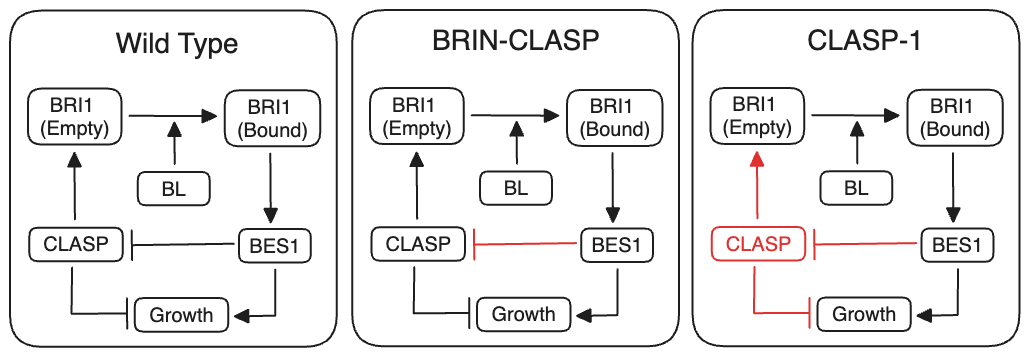
\includegraphics[width=13cm]{mutant-diagram.png}
    \caption{Signalling network in the wild type, BRIN-CLASP mutant, and CLASP-1 mutant. Red arrows denote signalling pathways that were removed due to the mutation.} 
    \label{fig:mutant-diagram}
\end{figure}


\begin{equation}
\label{column-equations}
\begin{aligned}
    &\frac{dL_{\text{C1}}}{dt} = ((g_{0} - 0) + R_{\text{C1}}P)L, &\frac{dD}{dt} = d_{0}\left( 1 - \frac{L^{n}}{d_{L}^{n} + L^{n}} \right)  \\[5pt]
    &\frac{dL_{\text{BC}}}{dt} = ((g_{0} - C_{\text{BC}}) + R_{\text{BC}}P)L, &\frac{dD}{dt} = d_{0}\left( 1 - \frac{L^{n}}{d_{L}^{n} + L^{n}} \right)  \\[5pt]
    &\frac{dL_{\text{WT}}}{dt} = ((g_{0} - C_{\text{WT}}) + R_{\text{WT}}P)L,  &\frac{dD}{dt} = d_{0}\left( 1 - \frac{L^{n}}{d_{L}^{n} + L^{n}} \right)
\end{aligned}
\end{equation}


\medskip

As discussed previously, these equations are subject to the restrictions $0 < C_{\text{WT}} < C_{\text{BC}}$ and $R_{\text{C1}} < R_{\text{WT}} < R_{\text{BC}}$. We ran the model with a time step $0.01$ for a period of $T = 500$ arbitrary units. The simulations were initialized with $10$ cells of length $7\um$. Parameters were fitted by hand to match an exponential curve fitted to experimentally observed data. The results of these simulations are shown in Figure \ref{fig:column-position-length}. For more information, see the supplementary figures in the appendix. The parameters used in all of the figures presented are shown in Table \ref{tab:cell-column-parameters} while information about division behaviour is shown in Table \ref{tab:cell-column-divisions}.


\begin{table}
    \begin{center}
        \begin{tabular}{ |c|c|c| }
        \hline
         Parameter & Units & Value \\
         \hline
         $g_{0}$ & $1/t$ & $0.02500$ \\ 
         $c_{\text{WT}}$ & $1/t$ & $0.01400$ \\ 
         $c_{\text{BC}}$ & $1/t$ & $0.02200$ \\ 
         $R_{\text{C1}}$ & $1/(\um \cdot t)$ & $0.00028$ \\ 
         $R_{\text{WT}}$ & $1/(\um \cdot t)$ & $0.00029$ \\ 
         $R_{\text{BC}}$ & $1/(\um \cdot t)$ & $0.00030$ \\ 
         $d_{0}$ & $D/t$ & $0.05000$ \\ 
         $d_{L}$ & $\um$ & $20.0000$ \\ 
         $n$ & $1$ & $20.0000$ \\ 
         \hline
        \end{tabular}
    \caption{Parameter values for cell column model.}
    \label{tab:cell-column-parameters}
    \end{center}
\end{table}

\begin{table}
    \begin{center}
        \begin{tabular}{ |c|c|c|c|c| } 
        \hline
        Model & Mean Div. & Median Div. & Max Div. & \# Divs.  \\
        \hline
        Wild Type & $158.51$ & $151.41$ & $344.34$ & $537$  \\
        BRIN-CLASP & $138.26$ & $131.49$ & $307.45$ & $523$  \\
        CLASP-1 & $96.28$ & $83.80$ & $241.98$ & $396$  \\
        \hline
        \end{tabular}
    \caption{Division behaviour in cell column models.}
    \label{tab:cell-column-divisions}
    \end{center}
\end{table}

\medskip

\begin{figure}
    \centering
    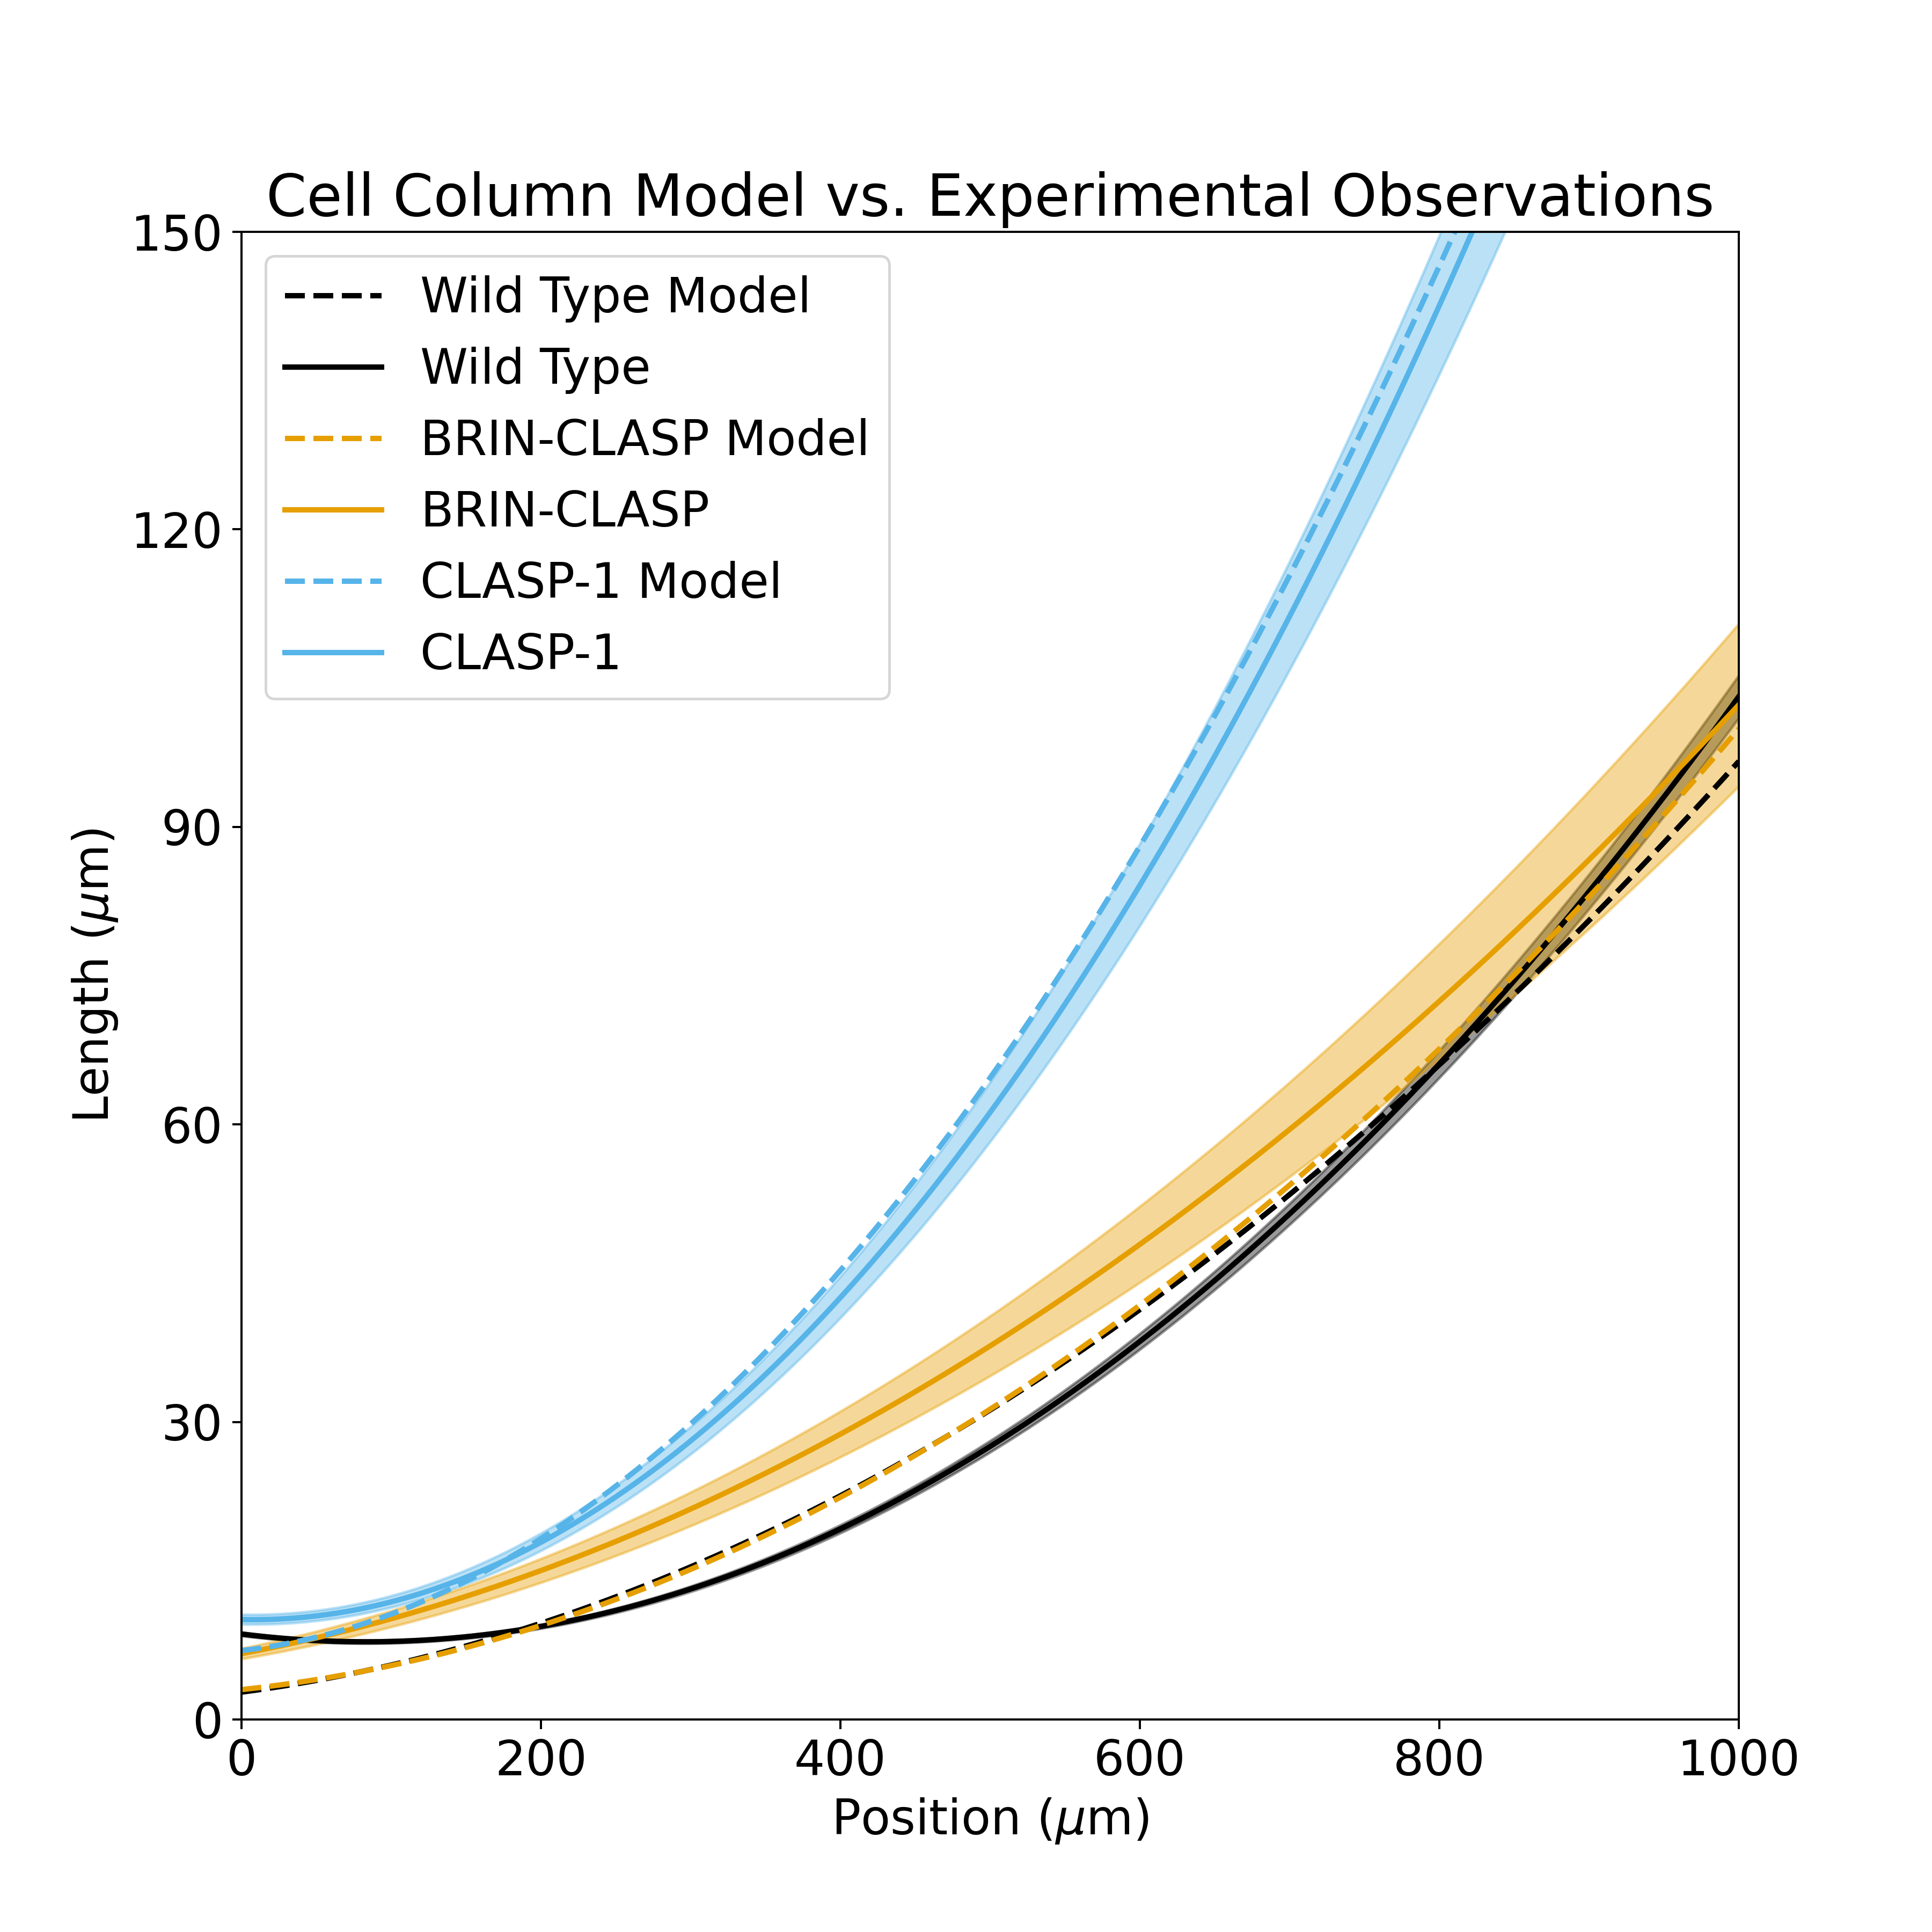
\includegraphics[width=13cm]{column-position-length.png}
    \caption{Position vs. length data from the model compared with experimental observations.}
    \label{fig:column-position-length}
\end{figure}



\newpage

\section{Single Cell BES1 Model}

\subsection{Brassinoslide Component}

\cite{vukasinovic2021} provide a detailed biosynthetic pathway for BL by outlining how campestrol undergoes multiple chemical reactions to eventually form BL. The biosynthetic enzymes DWF4, CPD, DET3, ROT3, BR6OX1, and BR6OX2 catalyze these reactions. Mutants made to be deficient in each of the aforementioned enzymes exhibited stunted growth, which shows that these enzymes are crucial for effective BL synthesis. The biosynthetic enzymes CPD and ROT3 were observed by \cite{vukasinovic2021} using fluorescence imaging in the vascular cell columns of a single root. They found that both CPD and ROT3 remain relatively constant in the meristem (0-200\um) before increasing in the transition zone (200-400\um) and reaching a maximum in the early elongation zone (400-700\um). After 700\um, the CPD and ROT3 levels began to decrease.

\medskip

Since BL is the most biosynthetically active brassinosteroid, we make the assumption that it is the only brassinosteroid present in the root. Additionally, we assume that the fluorescence intensity of CPD and ROT3 measured by (\cite{vukasinovic2021}) are equivalent to the concentration of BL ligand up to some scalar multiple. To determine this scalar, we use an estimate from \cite{vanesse2012} that gives the extracellular concentration of BL ligand to be at most 1\nm in wild-type roots. This gives us the following formula for the extracellular BL concentration [BL] in \nm:

\begin{equation}
    \label{bl}
[\text{BL}] = b \cdot \frac{\text{CPD}}{\text{max}(\text{CPD})} + (1 - b) \cdot \frac{\text{ROT3}}{\text{max}(\text{ROT3})}
\end{equation}

\medskip

In \eqref{bl}, the parameter $b \in [0, 1]$ controls the bias towards CPD in order to account for the fact that the exact details of the BL pathway are omitted from our model. Using the data from \cite{vukasinovic2021} along with \eqref{bl}, we plotted the BL concentration against position for different levels of bias (see Supplementary Figure \ref{sfig:bl-bias}). Since the functions behaved qualitatively the same, we assigned $b = 0.5$. Additionally, BR biosynthetic enzymes have been shown to move short distances in the root (\cite{vukasinovic2021}), so we take an $n\,\um$ moving average of the BL concentration function to account for diffusion. Shown in Supplementary Figure \ref{sfig:bl-average} is a plot of the BL concentration function for different values of $n$. We settled on $n = 50\um$ as a reaosnable estimate of this diffusive effect.


\subsection{BRI1 Receptor Component}

From the description of the BL concentration function in Equation \eqref{bl} we can derive a formula for the concentration of bound BRI1 receptors at any position in the root. To do this, we use the equilibrium and mass-balance equations for the BRI1 receptor network introduced by \cite{vanesse2012}.

\begin{equation}
    \label{eq}
    [\text{BRI1 BL}] = \frac{[\text{BRI1}_{\text{free}}] \cdot [\text{BL}_{\text{free}}]}{K_{d}}
\end{equation}

\begin{equation}
    \label{mb}
\begin{aligned}
    \relax
    [\text{BRI1}] &= [\text{BRI1 BL}] + [\text{BRI1}_{\text{free}}]\\[5pt]
    [\text{BL}] &= [\text{BRI1 BL}] + [\text{BL}_{\text{free}}]
\end{aligned}
\end{equation}

In the equations above, $[\text{BRI1 BL}]$ denotes the concentration of bound BRI1 receptors, which are assumed to bind at a ratio of one molecule to one monomer (\cite{vanesse2012}). $K_{d}$ is the BL dissociation constant. Additionally, $[\text{BRI1}_{\text{free}}]$ and $[\text{BL}_{\text{free}}]$ denote the unbound BRI1 and BL concentrations respectively, while $[\text{BL}]$ and $[\text{BRI1}]$ represent the total BRI1 and BL concentrations. To further simplify our model, we can express $[\text{BRI1 BL}]$ as a function of $[\text{BRI1}]$ and $[\text{BL}]$ by substituting \eqref{mb} into \eqref{eq} to get:


\begin{equation}
\label{bri1-1}
[\text{BRI1 BL}] = \frac{([\text{BRI1}] - [\text{BRI1 BL}])([\text{BL}] - [\text{BRI1 BL}])}{K_{d}}
\end{equation}

\begin{equation}
\label{bri1-2}
K_{d} \cdot [\text{BRI1 BL}] = [\text{BRI1}] \cdot [\text{BL}] - ([\text{BL}] + [\text{BRI1}]) \cdot [\text{BRI1 BL}] + [\text{BRI1 BL}]^{2}
\end{equation}

\begin{equation}
\label{bri1-3}
[\text{BRI1 BL}]^{2} - ([\text{BL}] + [\text{BRI1}] + K_{d}) \cdot [\text{BRI1 BL}] + ([\text{BRI1}] \cdot [\text{BL}]) = 0
\end{equation}

Now, we can use the quadratic formula to determine the positive value of $[\text{BRI1 BL}]$ for which \eqref{bri1-3} holds. This gives us a formula for $[\text{BRI1 BL}]$ in terms of $[\text{BRI1}]$ and $[\text{BR}]$, where $A = ([\text{BL}] + [\text{BRI1}] + K_{d})$.

\begin{equation}
\label{bri1}
[\text{BRI1 BL}] = \frac{A - \sqrt{A^{2} - 4 \cdot [\text{BRI1}] \cdot [\text{BL}]}}{2}
\end{equation}

Empirical research gives us estimates for the values of $[\text{BRI1}]$ and $K_{d}$. \cite{vanesse2012} estimate the BRI1 receptor concentration to be $62 \pm 4 \nm$ in wild type roots. Values for the BL dissociation constant $K_{d}$ range from $7.4 \nm$ to $15 \nm$ (\cite{wang2001}) up to $55 \nm$ (\cite{cano-delgado2004}). For the models presented in the forthcoming sections, we will take $[\text{BRI1}] = 62 \nm$  and $K_{d} = 10\nm$. Using these parameters along with the formula in equation \eqref{bri1} we get the $[\text{BRI1 BL}]$ function shown in Figure \ref{fig:bri1-function}.

\begin{figure}
    \centering
    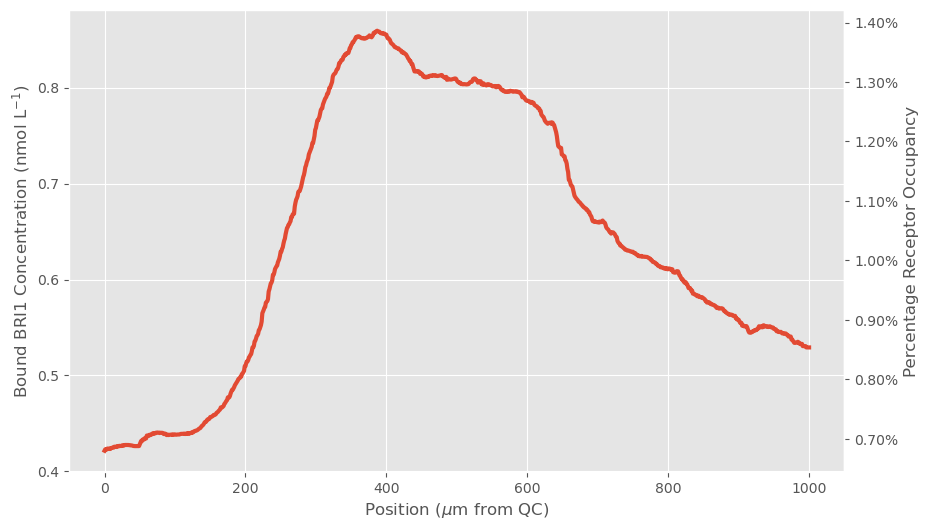
\includegraphics[width=13cm]{img/bri1-function.png}
    \caption{Plot of bound receptor concentration (left axis) measured in $\nm$ as well as receptor occupancy percentage (right axis). Due to the fact that $[\text{BL}] \ll [\text{BRI1}]$ the $[\text{BRI1 BL}]$ function is approximately equal to the $[\text{BL}]$ function up to some scalar multiple. }
    \label{fig:bri1-function}
\end{figure}


\medskip

Our model makes the assumption that all BRI1 receptors are localized to the cell membrane. Additionally, it assumes that the law of mass action is a reasonable approximation for the diffusing BL ligand binding to the static BRI1 receptors. We believe this decision is justified due to the low percentage occupancy of the BRI1 receptors, which suggests that any free BL ligand will have many oppourtunities to bind to a receptor. Further modelling of the BRI1 receptor network using the physical properties of the system would help to clarify and refine these assumptions.



\subsection{BES1 Signalling Model} \label{bes1-model-section}

In this model and all subsequent models we aim to predict the behaviour of a single cell as it is pushed away from the quiescent centre (henceforth QC) by the growth and division of the cells beneath it. Within the meristematic zone, cells grow from a length of $4.5\um$ to $9\um$ over a period of approximately $18\h$ (\cite{verbelen2006}). However, cells may undergo one or more divisions during this time (\cite{goh2023}), so tracking the exact lineage of a single cell is difficult. For this reason, our model will only consider cells at $150\um$ or higher above the QC. 

\medskip

Prior to writing down a system of differential equations for our model, we need to rescale our data to be in terms of time instead of position. To do this, we map a position of $150\um$ above the QC to $t = 0\h$ and then use cell lineage data from \cite{goh2023} to determine a function that maps positions to times. The resulting position function is shown in Supplementary Figure \ref{sfig:position-function}.

\medskip

Our first model aims to predict the level of BR signalling within the cell as it moves away from the QC, measured in terms of the BES1 transcription factor. To do this, we will use a time-rescaled version of the BL concentration function shown in Supplementary Figures \ref{sfig:bl-bias} and \ref{sfig:bl-average} with $b = 0.5$ and $n = 50$. The model will be fit to time-rescaled fluorescence intensity data from the cell columns of a single \emph{A. thaliana} root (\cite{vukasinovic2021}). The BL concentration function and the data are shown in Supplementary Figure \ref{sfig:bes1-data}. It is important to note that there is likely additional plant-to-plant variance that remains unaccounted for due to the fact that the data comes from a single organism. 

\medskip

With our data prepared, we can now define an ODE model for the amount of BES1 transcript in terms of the BL concentration $B(t) = [\text{BL}]$. To do this, recall that Equation \eqref{bri1} gives us the concentration of bound BRI1 receptors $R_{B} = [\text{BRI1 BL}]$ in terms of $B(t)$, the dissociation constant $K_{d}$, and the total BRI1 concentration $R_{T} = [\text{BRI1}]$. For this model, we will fix $K_{d} = 10\nm$ (\cite{wang2001}) and $R_{T} = 62\nm$ (\cite{vanesse2012}) as in Figure \ref{fig:bri1-function}.

\begin{equation}
\label{rb}
R_{B}(B, R_{T}, K_{d}) = \frac{(B + R_{T} + K_{d}) - \sqrt{(B + R_{T} + K_{d})^{2} - 4 \cdot R_{T} \cdot B}}{2}
\end{equation}


When the concentration of bound BRI1 receptors $R_{B}$ is higher, the effects of the BIN2 signalling inhibitor are released, leading to increased production of BES1. Let $s_{\text{in}}$ denote the rate at which $R_{B}$ increases BES1 transcription. We also include a decay term with parameter $s_{\text{out}}$ to account for the degradation of the BES1 transcription factor over time. The intial condition is given by another parameter $\text{BES1}(0) = s_{0}$. Fitting this parameter will give us a non-dimensional estimate for the level of BES1 signalling at $150\um$ above the QC. 

\begin{equation}
\label{bes1}
\frac{d\text{BES1}}{dt} = s_{\text{in}}R_{B}(B, R_{T}, K_{d}) - s_{\text{out}}\text{BES1},\quad \text{BES1}(0) = s_{0}
\end{equation}

Since $R_{B}$ has $t$-dependence through the BL concentration function $B$, Equation \eqref{bes1} cannot be solved analytically and must be approximated using numerical methods. Before we show the results of these simulations, we present a visual summary of the model in Figure \ref{fig:bes1-model}.

\begin{figure}
    \centering
    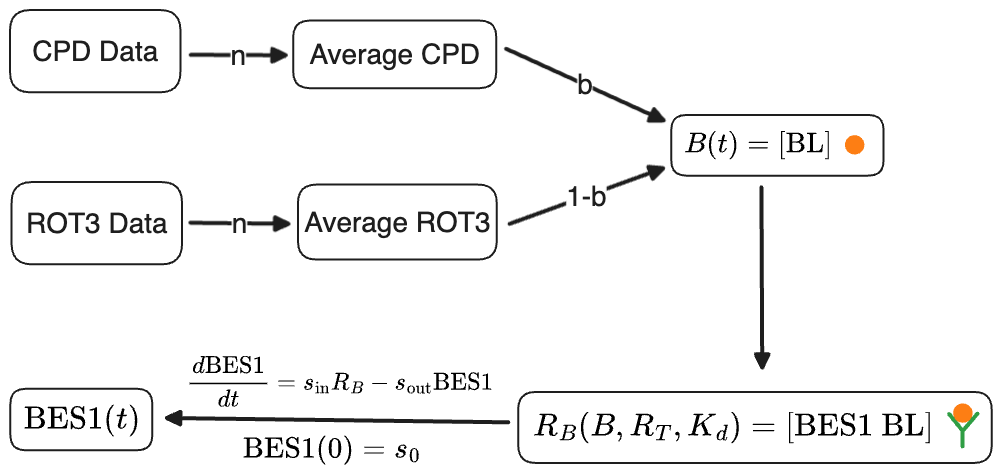
\includegraphics[width=13cm]{bes1-model.png}
    \caption{A visual depiction of the model up to this point. The extracellular BL concentration function $B(t)$ is computed using a moving biased average of the CPD and ROT3 biosynthetic enzymes. Then, $B(t)$ is used to determine the concentration of bound receptors $R_{B}$, building on the work of \cite{vanesse2012}. Finally, an ordinary differential equation model is used to express the BES1 transcription factor as a function of time through $R_{B}$.}
    \label{fig:bes1-model}
\end{figure}

\medskip

The BES1 function was approximated using a forward euler method with a time step of $0.01\h$. We evaluated the model using the Root-Mean-Squared Error (RMSE) metric. The formula is given in Equation \eqref{rmse} where $N$ denotes the number of observations. Each $y_{i}$ ($1 \leq i \leq N$) represents an observed value while each $f(t_{i})$ denotes the model output at time $t_{i}$.

\begin{equation}
\label{rmse}
\text{RMSE} =  \sqrt{\frac{1}{N}\sum_{i = 1}^{N} (y_{i} - f(t_{i}))^{2}}
\end{equation}


Additionally, the Akaike Information Criterion (henceforth AIC) presented in \cite{akaike1974} was used to compare the model presented (henceforth referred to as the complete model) with a linear and exponential regression on the BES1 signalling data. The AIC compares the relative quality of statistical models by considering both the goodness of fit and the informational complexity of the model. 

\begin{equation}
\label{aic}
\Delta \text{AIC} = 2k + N \ln\left( \frac{1}{N} \sum_{i = 1}^{N} (y_{i} - f(t_{i}))^{2}  \right) 
\end{equation}

In the equation above, $k$ denote the number of parameters in the model and $N$ is the number of observations. Since the AIC is used to compare models its absolute value is irrelevant. Therefore, the $\Delta \text{AIC}$ values presented in the forthcoming plots may be rescaled by a fixed constant to improve readability. The \verb|scipy.optimize.minimize| function from the scientific computation package \href{https://scipy.org/}{scipy} was used to determine the values of $s_{0} \in [0, 0.5]$, $s_{\text{in}} \in [0, 0.5]$, and $s_{\text{out}} \in [0, 0.5]$ that yielded the lowest error. Searching a larger parameter space did not produce a better fit (not shown).  Figure \ref{fig:bes1-model-fit} compares the fitted model to the experimental data and Table \ref{bes1-model-parameters} presents the optimized parameters. 

\begin{figure}
    \centering
    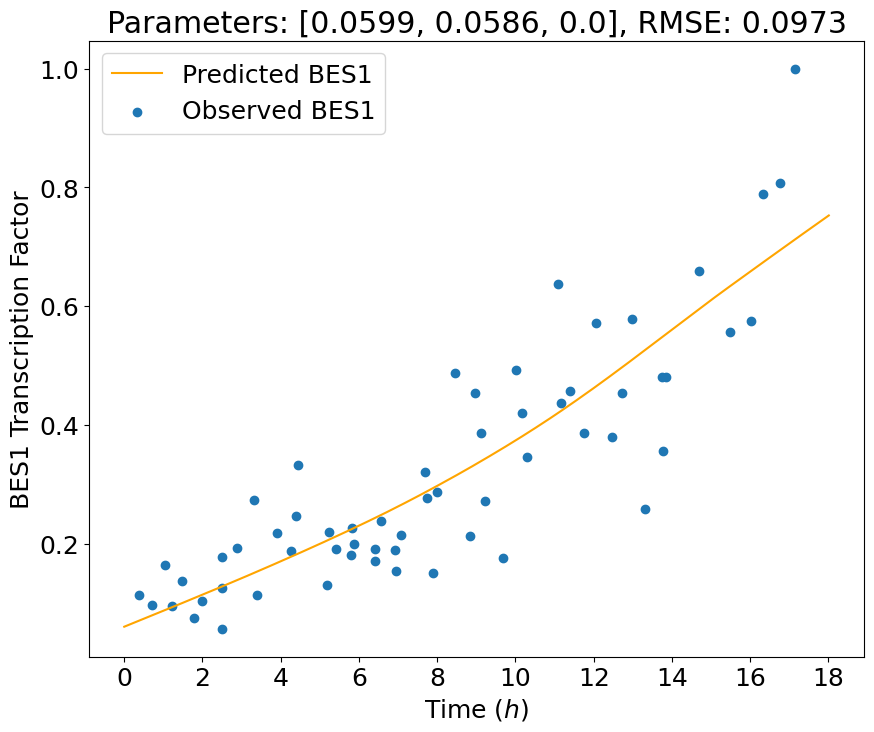
\includegraphics[width=13cm]{bes1-model-fit.png}
    \caption{Results of model fitting to the BES1 signalling data from \cite{vukasinovic2021}. The complete model was the best performing in terms of both absolute error and information-theoretic quality. } 
    \label{fig:bes1-model-fit}
\end{figure}

\medskip

\begin{center}
\label{bes1-model-parameters}
\begin{tabular}{ |c|c|c| } 
 \hline
 Parameter & Value & Units \\
 \hline
 $s_{0}$ & $2.35 \times 10^{-3}$ & $\text{BES1}$  \\
 $s_{\text{in}}$ & $4.79 \times 10^{-2}$ & $\text{BES1}/R_{B}\h$ \\ 
 $s_{\text{out}}$ & $3.53 \times 10^{-6}$ & $1/\h$ \\
 \hline
\end{tabular}
\end{center}

\medskip

The fitted parameter value $s_{\text{out}} = 3.53 \times 10^{-6}$ appears to be unreasonably low in the biological context of the problem. It suggests that BES1 has a half life of around $150$ days, which is unusually large. \cite{narsai2007} found that the the half life of transcription factors in \emph{A. thaliana} had a mean of $5.9\h$ and a median of $3.8\h$. However, some transcription factors had half lives above $24\h$. With these findings in mind, we can expect that the true value of $s_{\text{out}}$ is probably no more than $0.5$ and no less than $0.01$.

\medskip

To check if our model still performed reasonably well for values of $s_{\text{out}}$ within a biologically realistic range, we fixed $s_{0}$ to its fitted value and ran the model for a wide variety of possible $s_{\text{in}}$ and $s_{\text{out}}$ values. More precisely, we computed $100$ evenly spaced points from $s_{\text{in}} \in [0, 0.5]$ and $100$ evenly spaced points from $s_{\text{out}} \in [0, 0.5]$. This produced a lattice of $10\,000$ points in two-dimensional parameter space which were used to evaluate the model. Then, we ran the model at each of these points and plotted in the errors in Figure \ref{fig:bes1-model-heatmap}.

\begin{figure}
    \centering
    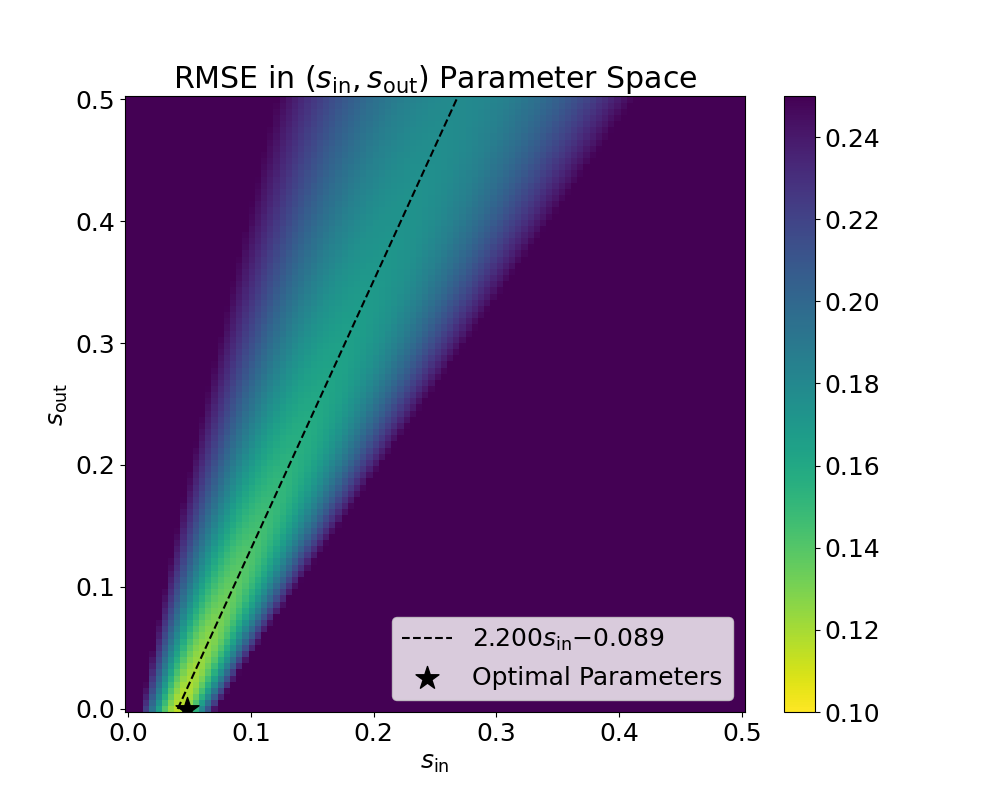
\includegraphics[width=13cm]{bes1-model-heatmap.png}
    \caption{Heatmap showing the model RMSE for a $100 \times 100$ grid of $(s_{\text{in}}, s_{\text{out}})$ parameter values. The initial condition $s_{0}$ was fixed to its fitted value of $2.35 \times 10^{-3}$. Regions of the plot shaded dark purple were truncated to an RMSE of $0.25$ and thus the actual RMSE at these points may be higher. The results of this process indicate a clear linear relationship between $s_{\text{in}}$ and $s_{\text{out}}$ which is given approximately by the linear function function $s_{\text{out}} = L(s_{\text{in}}) = 2.200s_{\text{in}} - 0.089$. }
    \label{fig:bes1-model-heatmap}
\end{figure}

\medskip

While the fitted parameter value $s_{\text{out}} = 3.53 \times 10^{-6}$ is probably not the true half life of the BES1 transcription factor as discussed previously, the parameter space search shows that the model also performs reasonably well for values of $s_{\text{out}}$ between $0.01$ and $0.5$. Lower values of $s_{\text{out}}$, which correspond with a longer BES1 half-life, produce slightly less error than higher values. This is indicated by the brighter yellow colour near the bottom of the dotted black line in Figure \ref{fig:bes1-model-heatmap}. In the regime where $s_{\text{out}}$ is small Equation \eqref{bes1} can be approximated as follows:


\begin{equation}
\label{bes1-sout-small}
\frac{\text{BES1}}{dt} = s_{\text{in}}R_{B} - s_{\text{out}}\text{BES1} \approx s_{\text{in}}R_{B} \Rightarrow \text{BES1} \approx s_{\text{in}} \int R_{B} \, dt
\end{equation}

This approximation indicates that the BES1 transcription factor accumulates over time in the cell and does not reach the maximum steady state value imposed by $s_{\text{out}}$. All of the biologically reasonable values for $s_{\text{out}}$ fall under this regime. For the sake of comparison, let us also consider the region of our parameter space where $s_{\text{out}}$ is large, which produces a less accurate fit. Under this regime we have the following approximation for the BES1 function:
$$
\text{BES1} = \frac{s_{\text{in}}R_{B}}{s_{\text{out}}} + \left( s_{0} - \frac{s_{\text{in}}R_{B}}{s_{\text{out}}} \right) e^{-s_{\text{out}}\text{BES1}} \approx \frac{s_{\text{in}}R_{B}}{s_{\text{out}}}
$$

When $s_{\text{out}}$ is large, the BES1 transcription factor rapidly reaches its steady state value, and is thus approximately proportional to $R_{B}$ over the domain. As mentioned previously, the actual system probably does not behaves this way since the model fits poorly to the data for larger values of $s_{\text{out}}$.

\medskip

The results of the parameter space search shown in Figure \ref{fig:bes1-model-heatmap} also indicate that if $s_{\text{in}}$ or $s_{\text{out}}$ can be determined through experiments, the other parameter value can also be estimated to a high degree of accuracy using the linear relationship $s_{\text{out}} = L(s_{\text{in}}) = 2.200s_{\text{in}} - 0.089$. This result is significant because it may be experimentally feasible to find $s_{\text{out}}$, the BES1 transcription factor decay constant, and use it to determine $s_{\text{in}}$, which would be difficult to determine experimentally. However, there are some caveats to this approach. Since the data has arbitrary units, quantifying $s_{\text{in}}$ would also require making exact measurements of the BES1 transcription factor and using them to rescale Equation \eqref{bes1} prior to using the linear relationship we identified. Additionally, there is some uncertainty in the behaviour of the BL concentration function $B(t)$ as the exact details of the BL biosynthetic pathway were left out of the model. That being said, the scale scale of the BL concentration ($\approx 1\nm$) is grounded in the literature (\cite{vanesse2012}). 


\newpage

\section{Single Cell Mutant Model}

%\subsection{Cell Growth Model}

The data presented in Figure \ref{fig:mutant-sizes} was transformed into units of time and length using the following procedure. First, we make the assumption that cells are perfect cylinders, so that their cross sectional area is equal to their length multiplied by their diameter. Then, we assume that the diameter of each cell is identical, and prescribe a suitably chosen $d$ based on experimental data (\cite{goh2023}). To convert cell number to position we take the cumulative sum of the cell lengths over each cell column. Missing data was filled in using the average length for that cell number. Finally, we use the the function shown in Figure \ref{fig:position-function} to transform the position series into a time series and plot it against the cell lengths. The results of this data preprocessing is shown in Figure \ref{fig:data-trichoblast}.

\begin{figure}[!hbt]
    \centering
    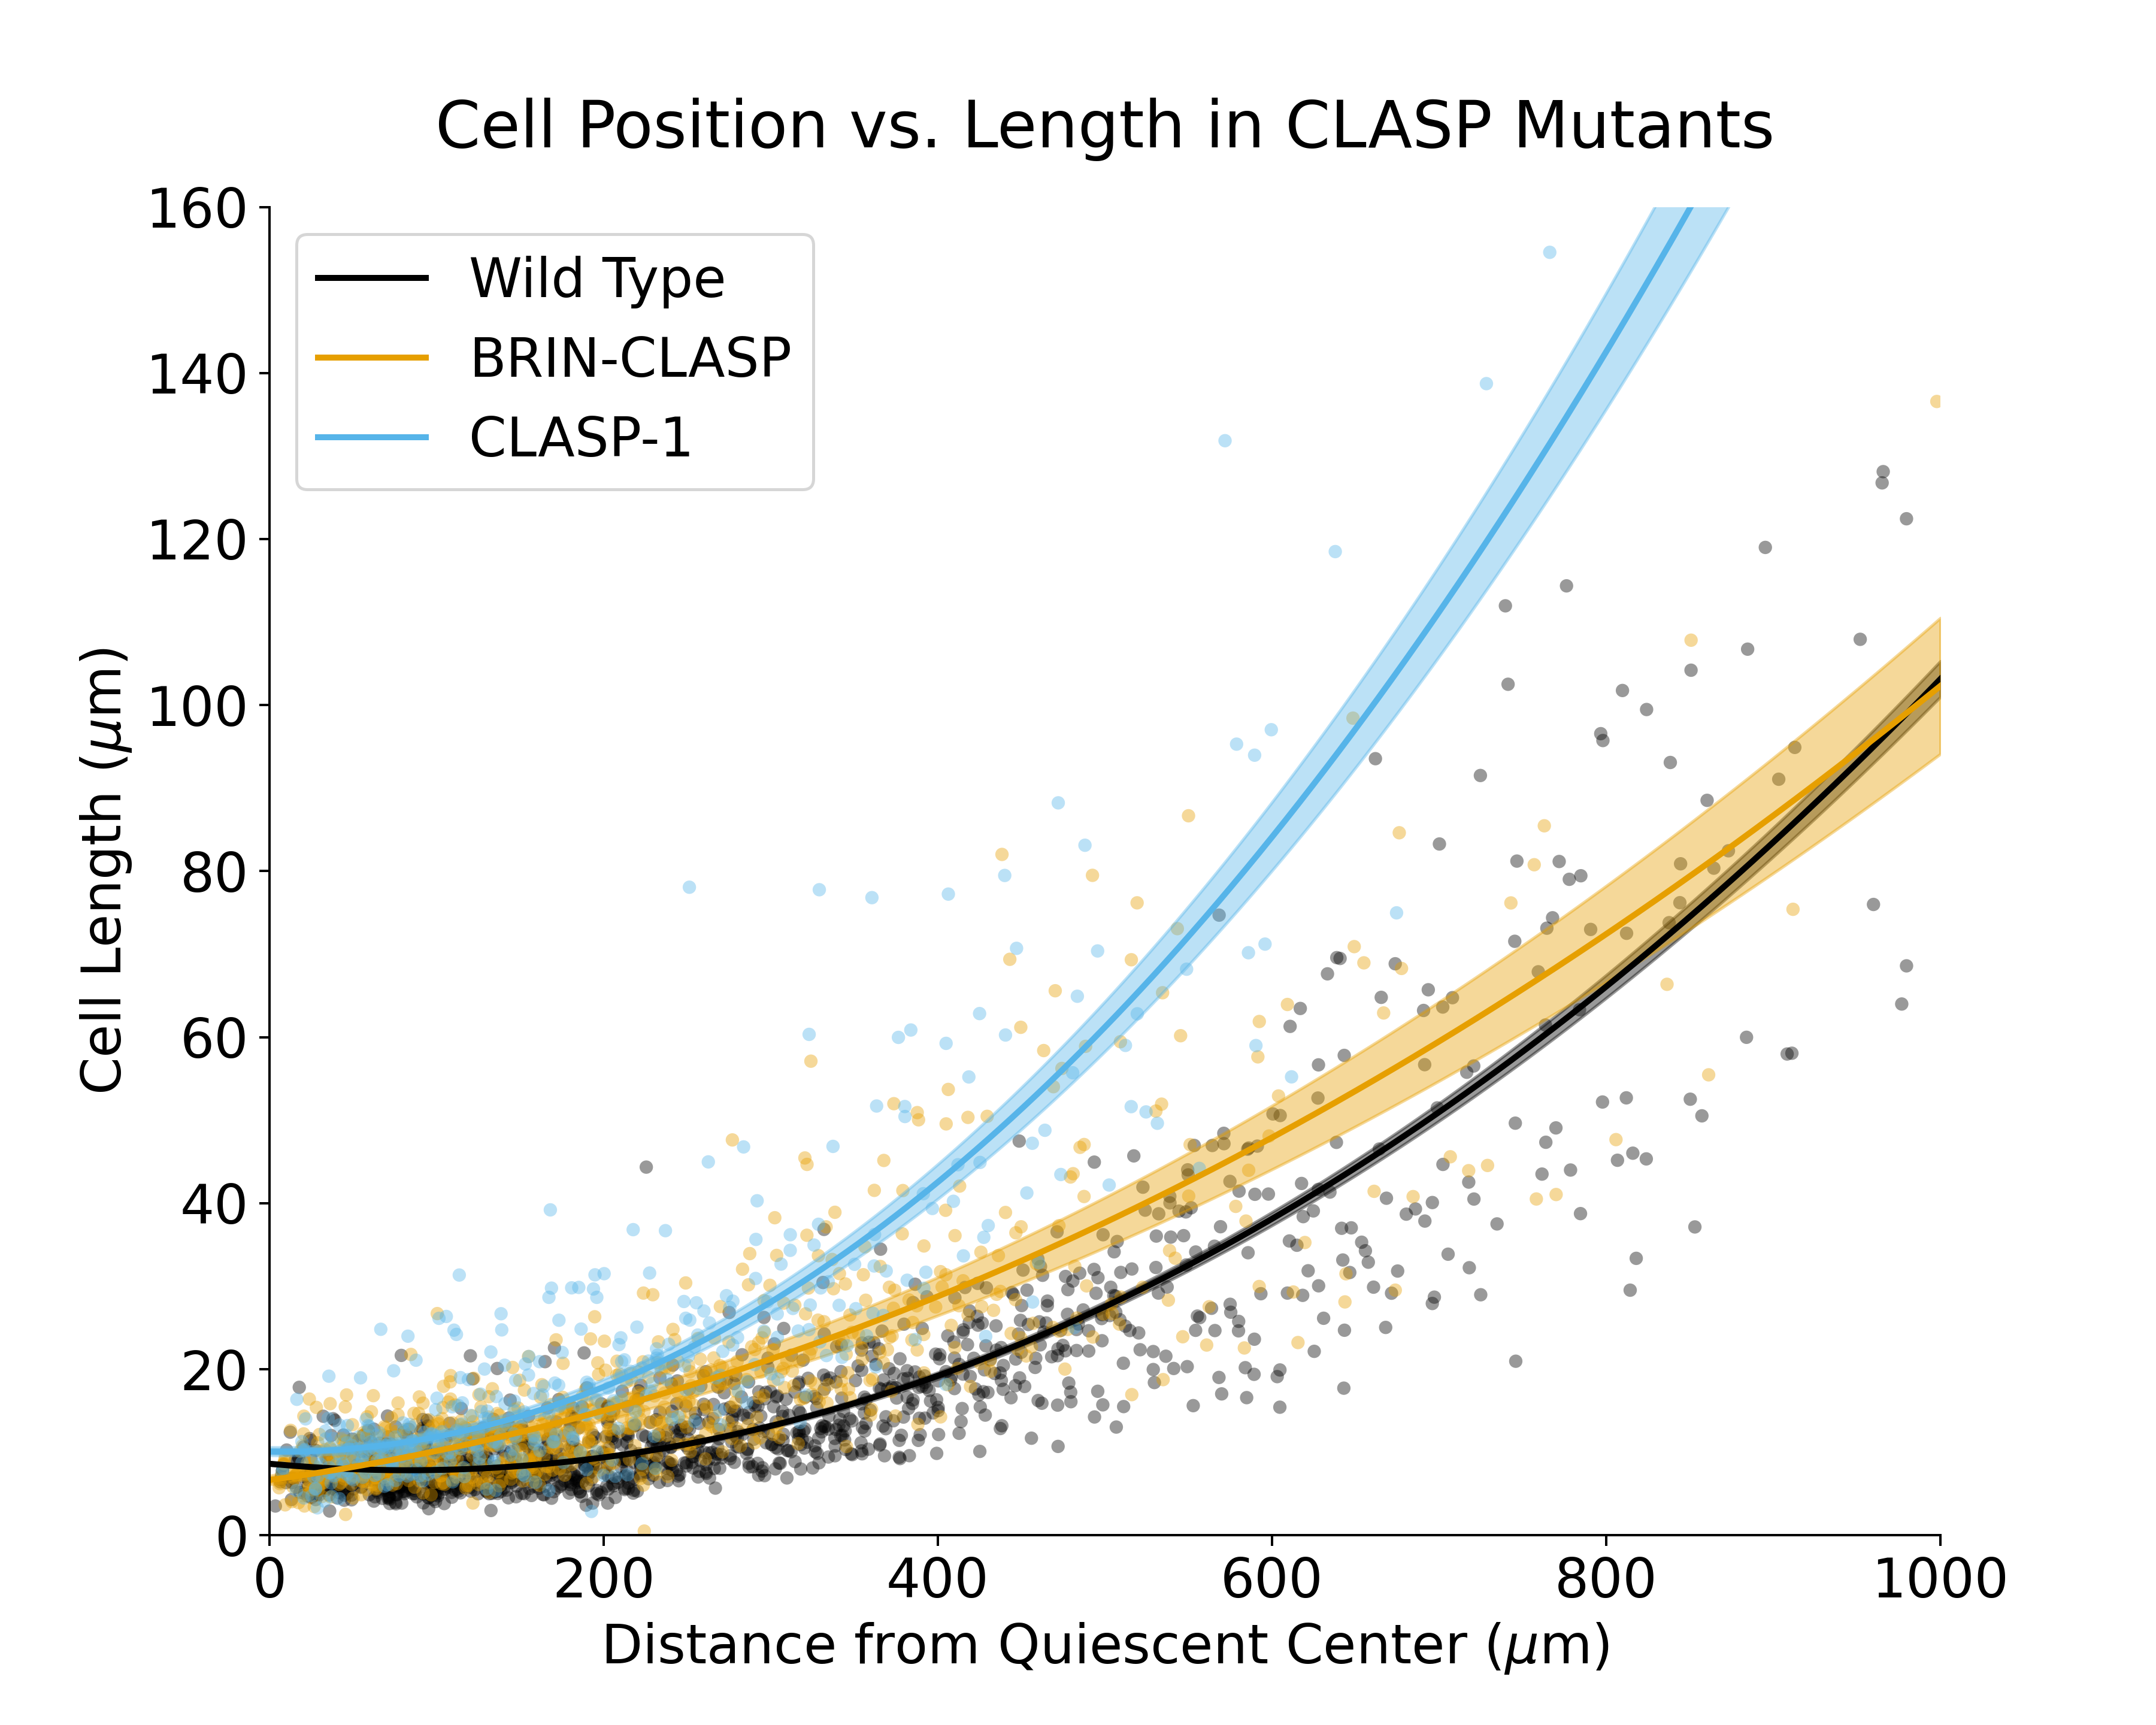
\includegraphics[width=13cm]{img/data-trichoblast.png}
    \caption{Plot of cell lengths from trichoblast cells in Wild Type, CLASP-1, and BRIN-CLASP roots. The line of best fit is an exponential function of the form $A + Be^{Cx}$. Wild Type cells are on average the shortest, followed closely by BRIN-CLASP. CLASP-1 cells are significantly longer, especially in the proximal regions of the root.}
    \label{fig:data-trichoblast}
\end{figure}

\medskip

While the model of cell growth presented here will consider exclusively wild type cells, later models will explore the CLASP-1 and BRIN-CLASP mutants. For reasons discussed later, the data we have available was insufficient for making quantitative modelling of the mutants. However, we do have enough information to verify that the mutants are indeed exhibiting different behaviour from the wild type. To do this, we compute the error of each data point from the line of best fit for the wild type cells. The distribution of these errors is shown in Figure \ref{fig:trichoblast-distribution}.

\begin{figure}
    \centering
    \label{fig:trichoblast-distribution}
    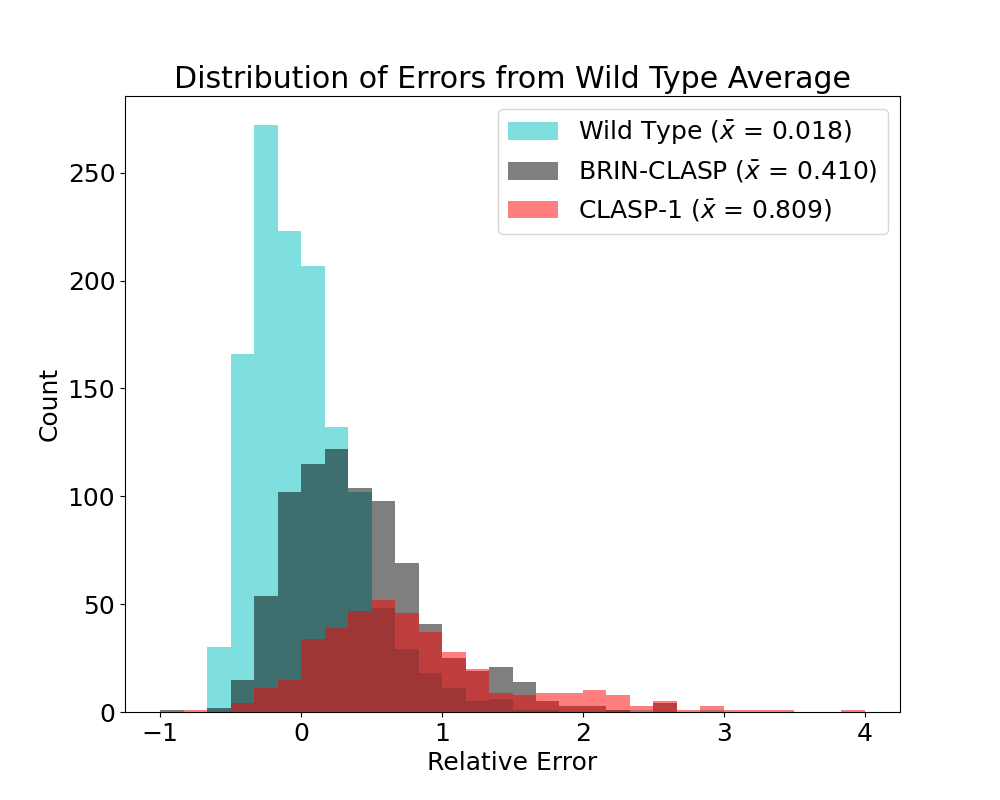
\includegraphics[width=13cm]{img/trichoblast-distribution.png}
    \caption{Distribution of errors from the wild type average presented in Figure \ref{fig:data-trichoblast}. The mean error of the BRIN-CLASP and CLASP-1 mutants are clearly positive, which suggests that the mutants have longer cells compared to the wild type. Both mutants had $p$-values less than $10^{-10}$ when compared to the wild type, which provides further evidence that the mutants are exhibiting different behaviour. }
\end{figure}


\medskip

For our first model of cell growth, we will consider exclusively wild type trichoblast cells. This model uses the ODE given in Equation \eqref{growth}, which is a variation on the model presented in \cite{lockhart1965} that accounts for the promotion of cell elongation by the BES1 transcription factor (\cite{vukasinovic2021}, \cite{ackerman-lavert2020}).

\begin{equation}
\label{growth}
\frac{dL}{dt} = (g_{P} + g_{B}\text{BES1})L
\end{equation}

In this model, $g_{P}$ denotes the basal growth rate due to the internal turgor pressure of the cell while $g_{B}$ denotes the rate at which $\text{BES1}$ promotes cell elongation. $\frac{dL}{dt}$ is scaled by the length $L$ because longer cells have more locations for the cellulose to stretch and reassemble (\cite{smithers2024}). An parameter corresponding to the initial condition $L(0) = g_{0}$ was also fitted. This parameter represents the average cell length at $150\um$ above the QC. 

\medskip

The BES1 equation \eqref{bes1} and length equation \eqref{growth} were approximated using a forward euler method with time step $0.01\ph$. Model fitting used the RMSE metric defined in equation \eqref{rmse} to fit the output to the data shown in Figure \ref{fig:data-trichoblast}. To reduce the dimensionality of the parameter space the parameters $s_{0}$, $s_{\text{in}}$, and $s_{\text{out}}$ from equation \eqref{bes1} were assigned their fitted values as shown in Figure \ref{fig:bes1-model-fit}. The parameter bounds used were $g_{0} \in [0, 10]$ and $g_{P}, g_{B} \in [0, 1]$. The results of the simulation are depicted in Figure \ref{fig:growth-model-fit}.

\begin{figure}[!hbt]
    \centering
    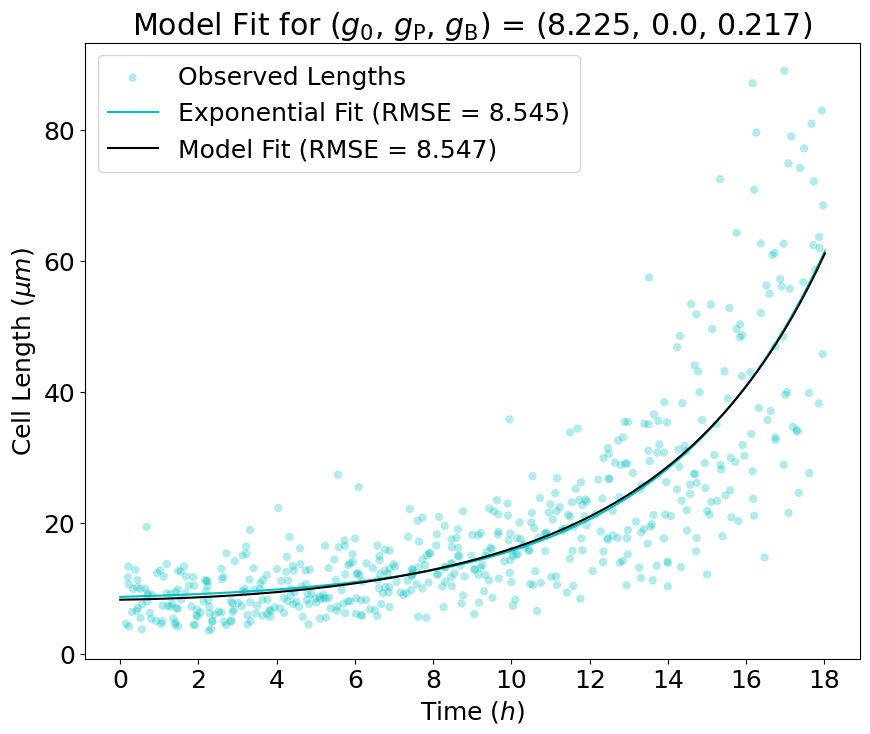
\includegraphics[width=13cm]{img/growth-model-fit.png}
    \caption{Results of fitting the growth model in equation \eqref{growth} to cell length data. The optimal parameter values were $g_{0} = 8.225\um$, $g_{P} = 0 \ph$ and $g_{B} = 0.0217\,\text{BES1}^{-1}\ph$. An exponential curve of the form $A + Be^{Cx}$ was also fitted to the data as a point of comparison. }
    \label{fig:growth-model-fit}
\end{figure}

\medskip

The result shown in Figure \ref{fig:growth-model-fit} suggests that our simple model is able to capture the trend in the data without invoking the existence of the CLASP protein. That being said, the abscence of the basal growth rate $g_{P}$ suggests that the optimal parameter values we found may not be representative of their true values. To get a better idea of the behaviour of our model we began by performing an uncertainty analysis. To do this, we  took each error $e_{i} = |f(t_{i}) - y_{i}|$, and then normalized it to get  the percentage error $\tilde{e_{i}} = e_{i} / y_{i}$. Then, we took the vectors of errors $\mathbf{e}$ and computed $1000$ random permutations $\mathbf{e}_{1}, \dots, \mathbf{e}_{1000}$. Finally, we constructed new $1000$ new data vectors $\mathbf{y}_{j} = f(\mathbf{t}) + \mathbf{e}_{j}$ and fitted the model to each one. The results of this analysis are shown in Figure \ref{fig:growth-model-uncertainty}.

\begin{figure}[!hbt]
    \centering
    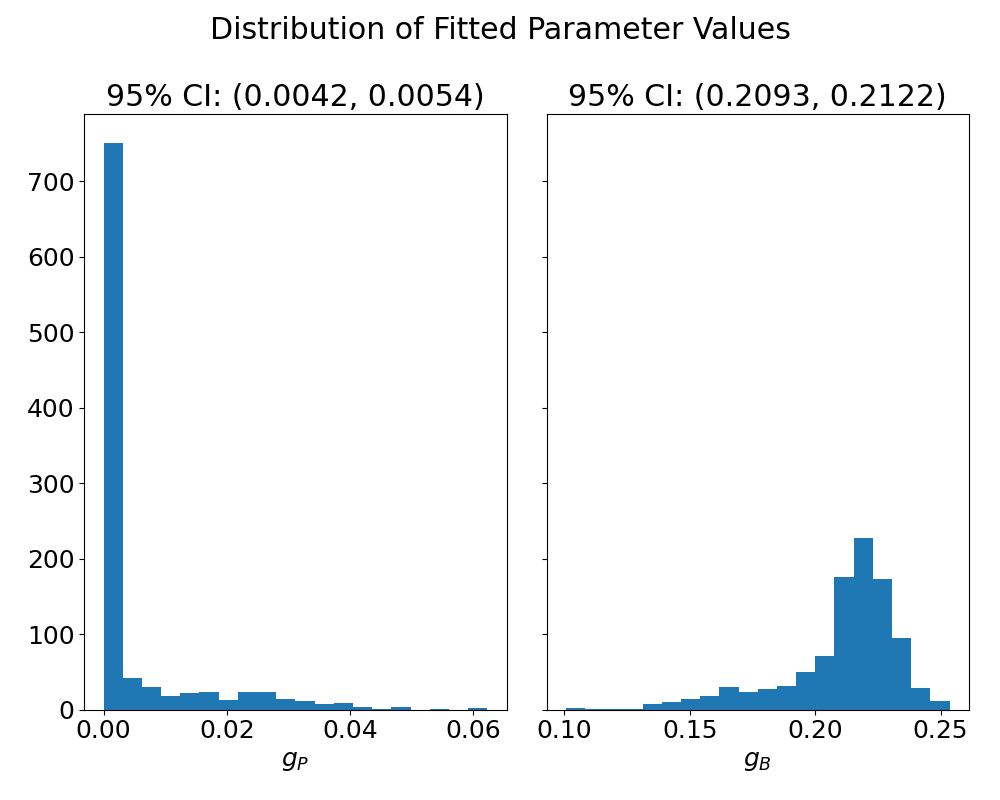
\includegraphics[width=13cm]{img/growth-model-uncertainty.png}
    \caption{A plot of the distribution of fitted $g_{P}$ and $g_{B}$ parameter values after the error shuffling process was repeated $1000$ times. Interestingly, the optimal parameters for the original data are outside the 95\% confidence intervals shown above. }
    \label{fig:growth-model-uncertainty}
\end{figure}

\medskip

A local sensitivity analysis over the domain $g_{P} \in [0, 0.1]$ and $g_{B} \in [0.1, 0.3]$ was also performed using the same methodologies described in Section \ref{bes1-model-section}. The results of this analysis are shown in Figure \ref{fig:growth-model-heatmap}.

\begin{figure}[!hbt]
    \centering
    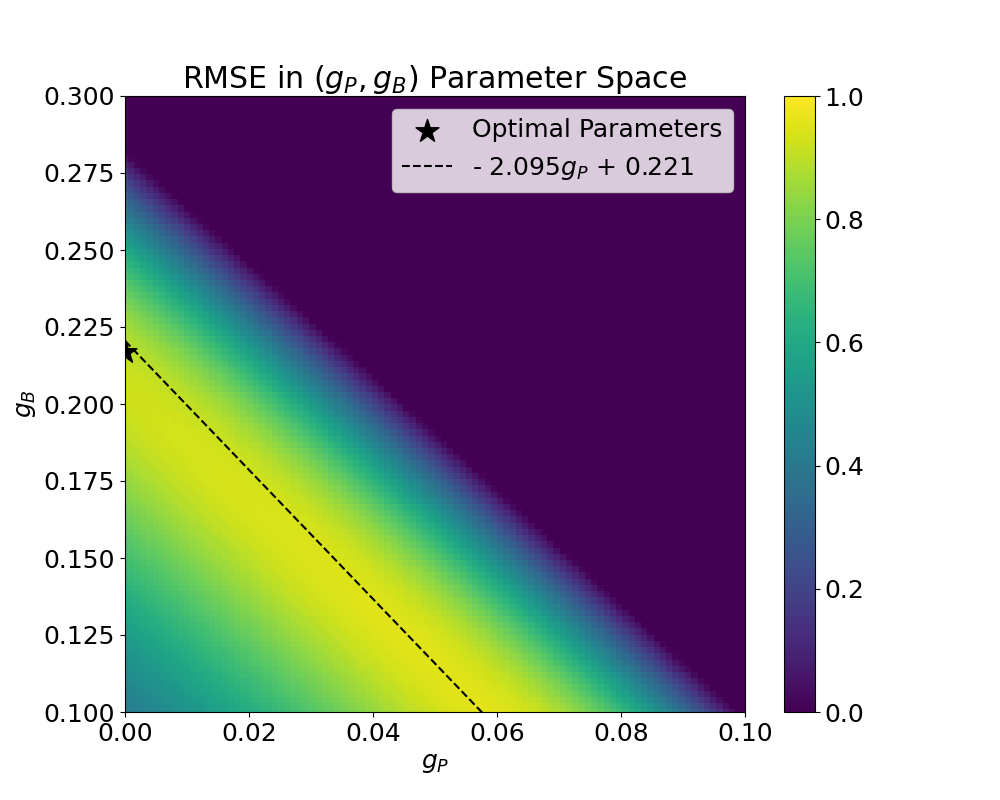
\includegraphics[width=13cm]{img/growth-model-heatmap.png}
    \caption{A heatmap of model error near the optimal parameter values $g_{P} = 0$ and $g_{B} = 0.217$. The RMSE remains low for values of $g_{B}$ and $g_{P}$ near the optimal range $g_{B} = -2.095g_{P} + 0.221$ but grows rapidly outside of that band. This result is not surprising given since if $g_{B}$ and $g_{P}$ are both high the model will overestimate the cell lengths. }
    \label{fig:growth-model-heatmap}
\end{figure}





% \subsection{CLASP-1 Mutant Model}

In this model, we introduce the CLASP protein to differentiate the wild type root from the CLASP-1 mutant. However, before we do this, it is necessary to confirm that the data from the mutant roots is different from the wild type. We do this by computing the percentage errors from the line of best fit for the wild type data shown in Figure \ref{fig:data-trichoblast}. Plotting these errors gives us a sampling distribution for all three types of roots (Wild Type, BRIN-CLASP, and CLASP-1) which we can compare using statistical methods.  These distributions are shown in Figure \ref{fig:trichoblast-distribution}.

\begin{figure}
    \centering
    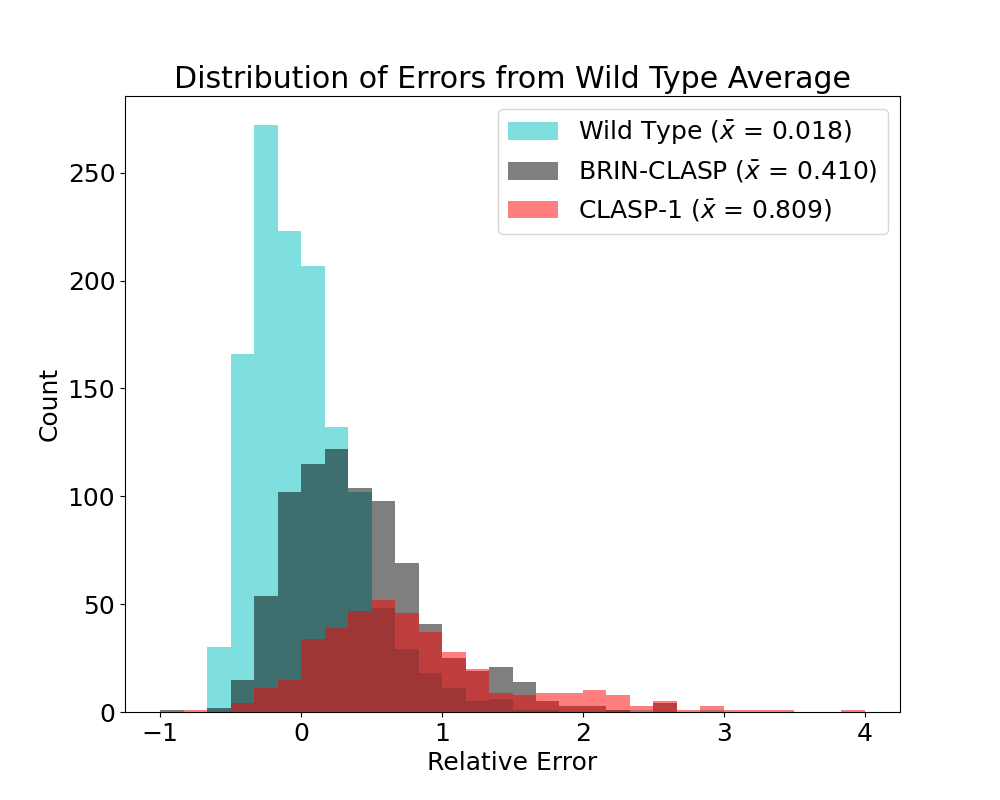
\includegraphics[width=13cm]{img/trichoblast-distribution.png}
    \caption{Distribution of errors from the wild type average presented in Figure \ref{fig:data-trichoblast}. The mean error of the BRIN-CLASP and CLASP-1 mutants are clearly positive, which suggests that the mutants have longer cells compared to the wild type. Both mutants had $p$-values less than $10^{-10}$ when compared to the wild type, which provides further evidence that the mutants are exhibiting different behaviour. }
    \label{fig:trichoblast-distribution}
\end{figure}


\medskip

Now that we have shown quantitatively that the wild type root is different from the CLASP-1 and BRIN-CLASP mutants we are ready to begin defining a system of ODEs for the CLASP-1 mutant model. First, assume that the CLASP protein $C$ is produced at a basal rate $c_{\text{in}}$. As discussed previously, the BES1 transcription factor inhibits CLASP by repressing its promoter (\cite{ruan2018}, so we include a parameter $c_{B}$ that represents this effect. We also include a background degradation rate $c_{\text{out}}$. Since $C$ will not be fitted to experimental data and is thus dimensionless, we will assign an initial condition of $C(0) = 1$. The differential equation defining the CLASP protein is shown in equation \eqref{clasp}.

\begin{equation}
\label{clasp}
\frac{dC}{dt} = c_{\text{in}} - (c_{\text{out}} + c_{B}\text{BES1})
\end{equation}

We also need to integrate the downstream effects of CLASP into our model. Experiments have found that CLASP inhibits growth in a length-dependent manner. Therefore, we add a $g_{C}C / L$ term to the denominator of  equation \eqref{growth} to get the modified version shown in equation \eqref{growth-clasp}. We also omit the $g_{P}$ parameter used in equation \eqref{growth} because this parameter was fit to $0$ in Figure \ref{fig:growth-model-fit}.

\begin{equation}
\label{growth-clasp}
\frac{dL}{dt} = \frac{(g_{B}\text{BES1})L}{1 + (g_{C}C/L)}
\end{equation}

An overview of the entire model incorporating BL, BRI1, BES1, CLASP, and cell growth is presented in Figure \ref{fig:clasp1-model}. The differential equations used in the model were approximated using a forward euler method with time step $0.01\h$. The model accuracy was quantified using the sum of the RMSE from the Wild Type and CLASP-1 data. In CLASP-1 roots we fixed the parameter values $c_{\text{in}} = c_{\text{out}} = c_{B} = 0$ and set the initial condition of the CLASP equation to $0$. Additionally, the CLASP-1 root is given a different initial length parameter $g_{1}$ that may differ from the initial length parameter $g_{0}$ used for the Wild Type.  All other parameters were held constant accross the two root types.

\begin{figure}
    \centering
    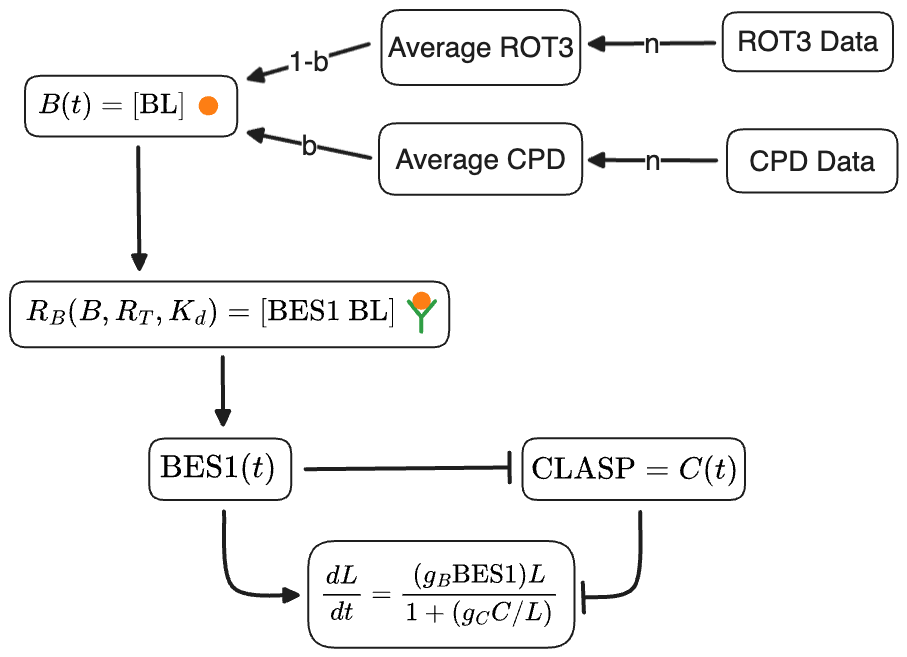
\includegraphics[width=13cm]{img/clasp1-model.png}
    \caption{Our complete model of cell growth in \emph{A. thaliana} which contains the BL concentration $B$, the BRI1 concentration $R_{T}$, the bound receptor concentration $R_{B}$, the level of $\text{BES1}$ signalling, the quantity of CLASP protein $C$, and the length of the cell $L$.}
    \label{fig:clasp1-model}
\end{figure}



% \subsection{BRIN-CLASP Model}


\newpage

\section{Discussion}


\subsection{The Single Cell Model}

Many of the parameters presented were prescribed or assigned prior to fitting the model. Some of these parameters, such as $K_{d}$ (the BL dissociation constant) and $R_{T}$ (the total concentration of BRI1 receptors) were based on previous results in the literature. However, other parameters such as $n$ (the BL moving average period) and $b$ (the CPD/ROT3 bias) were prescribed  with minimal justification. This was necessary due to the fact that the data available was only able to support a small number of parameters without running the risk of overfitting. In light of new data, it may be possible to get estimates and confidence intervals for the assigned parameters.

\medskip

Further experiments are necessary to more accurately fit the model. In particular, quantitative measurements of extracellular BR concentrations, CLASP protein levels, and the BES1 transcription factor would lead to significant improvements in model efficacy. The work in this paper also presents interesting oppourtunities for further modelling. Adding a model of cell division to the system of ODEs presented here would make it possible to describe an entire column of trichoblast or atrichoblast cells. This cell column model could be integrated into a two-dimensional cross section model (\cite{grieneisen2007}, \cite{dimambro2017}, \cite{salvi2020}), which often omit the effects of BR and CLASP on growth and division. This would make it possible to study the crosstalk between BR and auxin (\cite{chaiwanon2015}, \cite{vragovic2015}) \emph{in silico} to help us better understand how these crucial plant hormones interact with one another.

\subsection{Data Limitations}

% The descriptions and results from the additional models are contained in:
% - growth-model.tex
% - clasp1-model.tex
% - brin-clasp-model.tex

We developed models of cell growth using time-dependent ODEs but soon realized that such models could not be extended to the CLASP-1 and BRIN-CLASP mutants. The reason for this is that the data from \cite{goh2023} was crucial for converting position-dependent observations into time-dependent observations. However, this data was taken from wild type roots, and the position vs. time function we approximated is likely different for the mutants. In order to validate the time-dependent models presented in the previous section with experimental data, we would need multiple images of the CLASP-1 and BRIN-CLASP root tips over a period of time. Unfourtunately, this data is not currently available.




\appendix
\section{Supplementary Information}

\subsection{Quantifying Differences Between Mutants}

The raw data on the mutant roots presented in Figure \ref{fig:mutant-sizes} is in units of cell number versus cell length. The data was gathered from approximately $30$ cell columns per mutant, with each column originating from a different plant. We transformed this data into units of time and length using the following procedure. First, we made the assumption that cells are perfect cylinders, so that their cross sectional area is equal to their length multiplied by their diameter. Then, we assumed that the diameter of each cell is identical, and prescribed a suitably chosen diameter $d = 10\um$ based on experimental data (\cite{goh2023}). To convert cell number to position we took the cumulative sum of the cell lengths over each cell column. Missing data was filled in using the average length for that cell number and mutant. The results of this data preprocessing is shown in Figure \ref{sfig:data-trichoblast}.

\begin{supplementaryfigure}
    \centering
    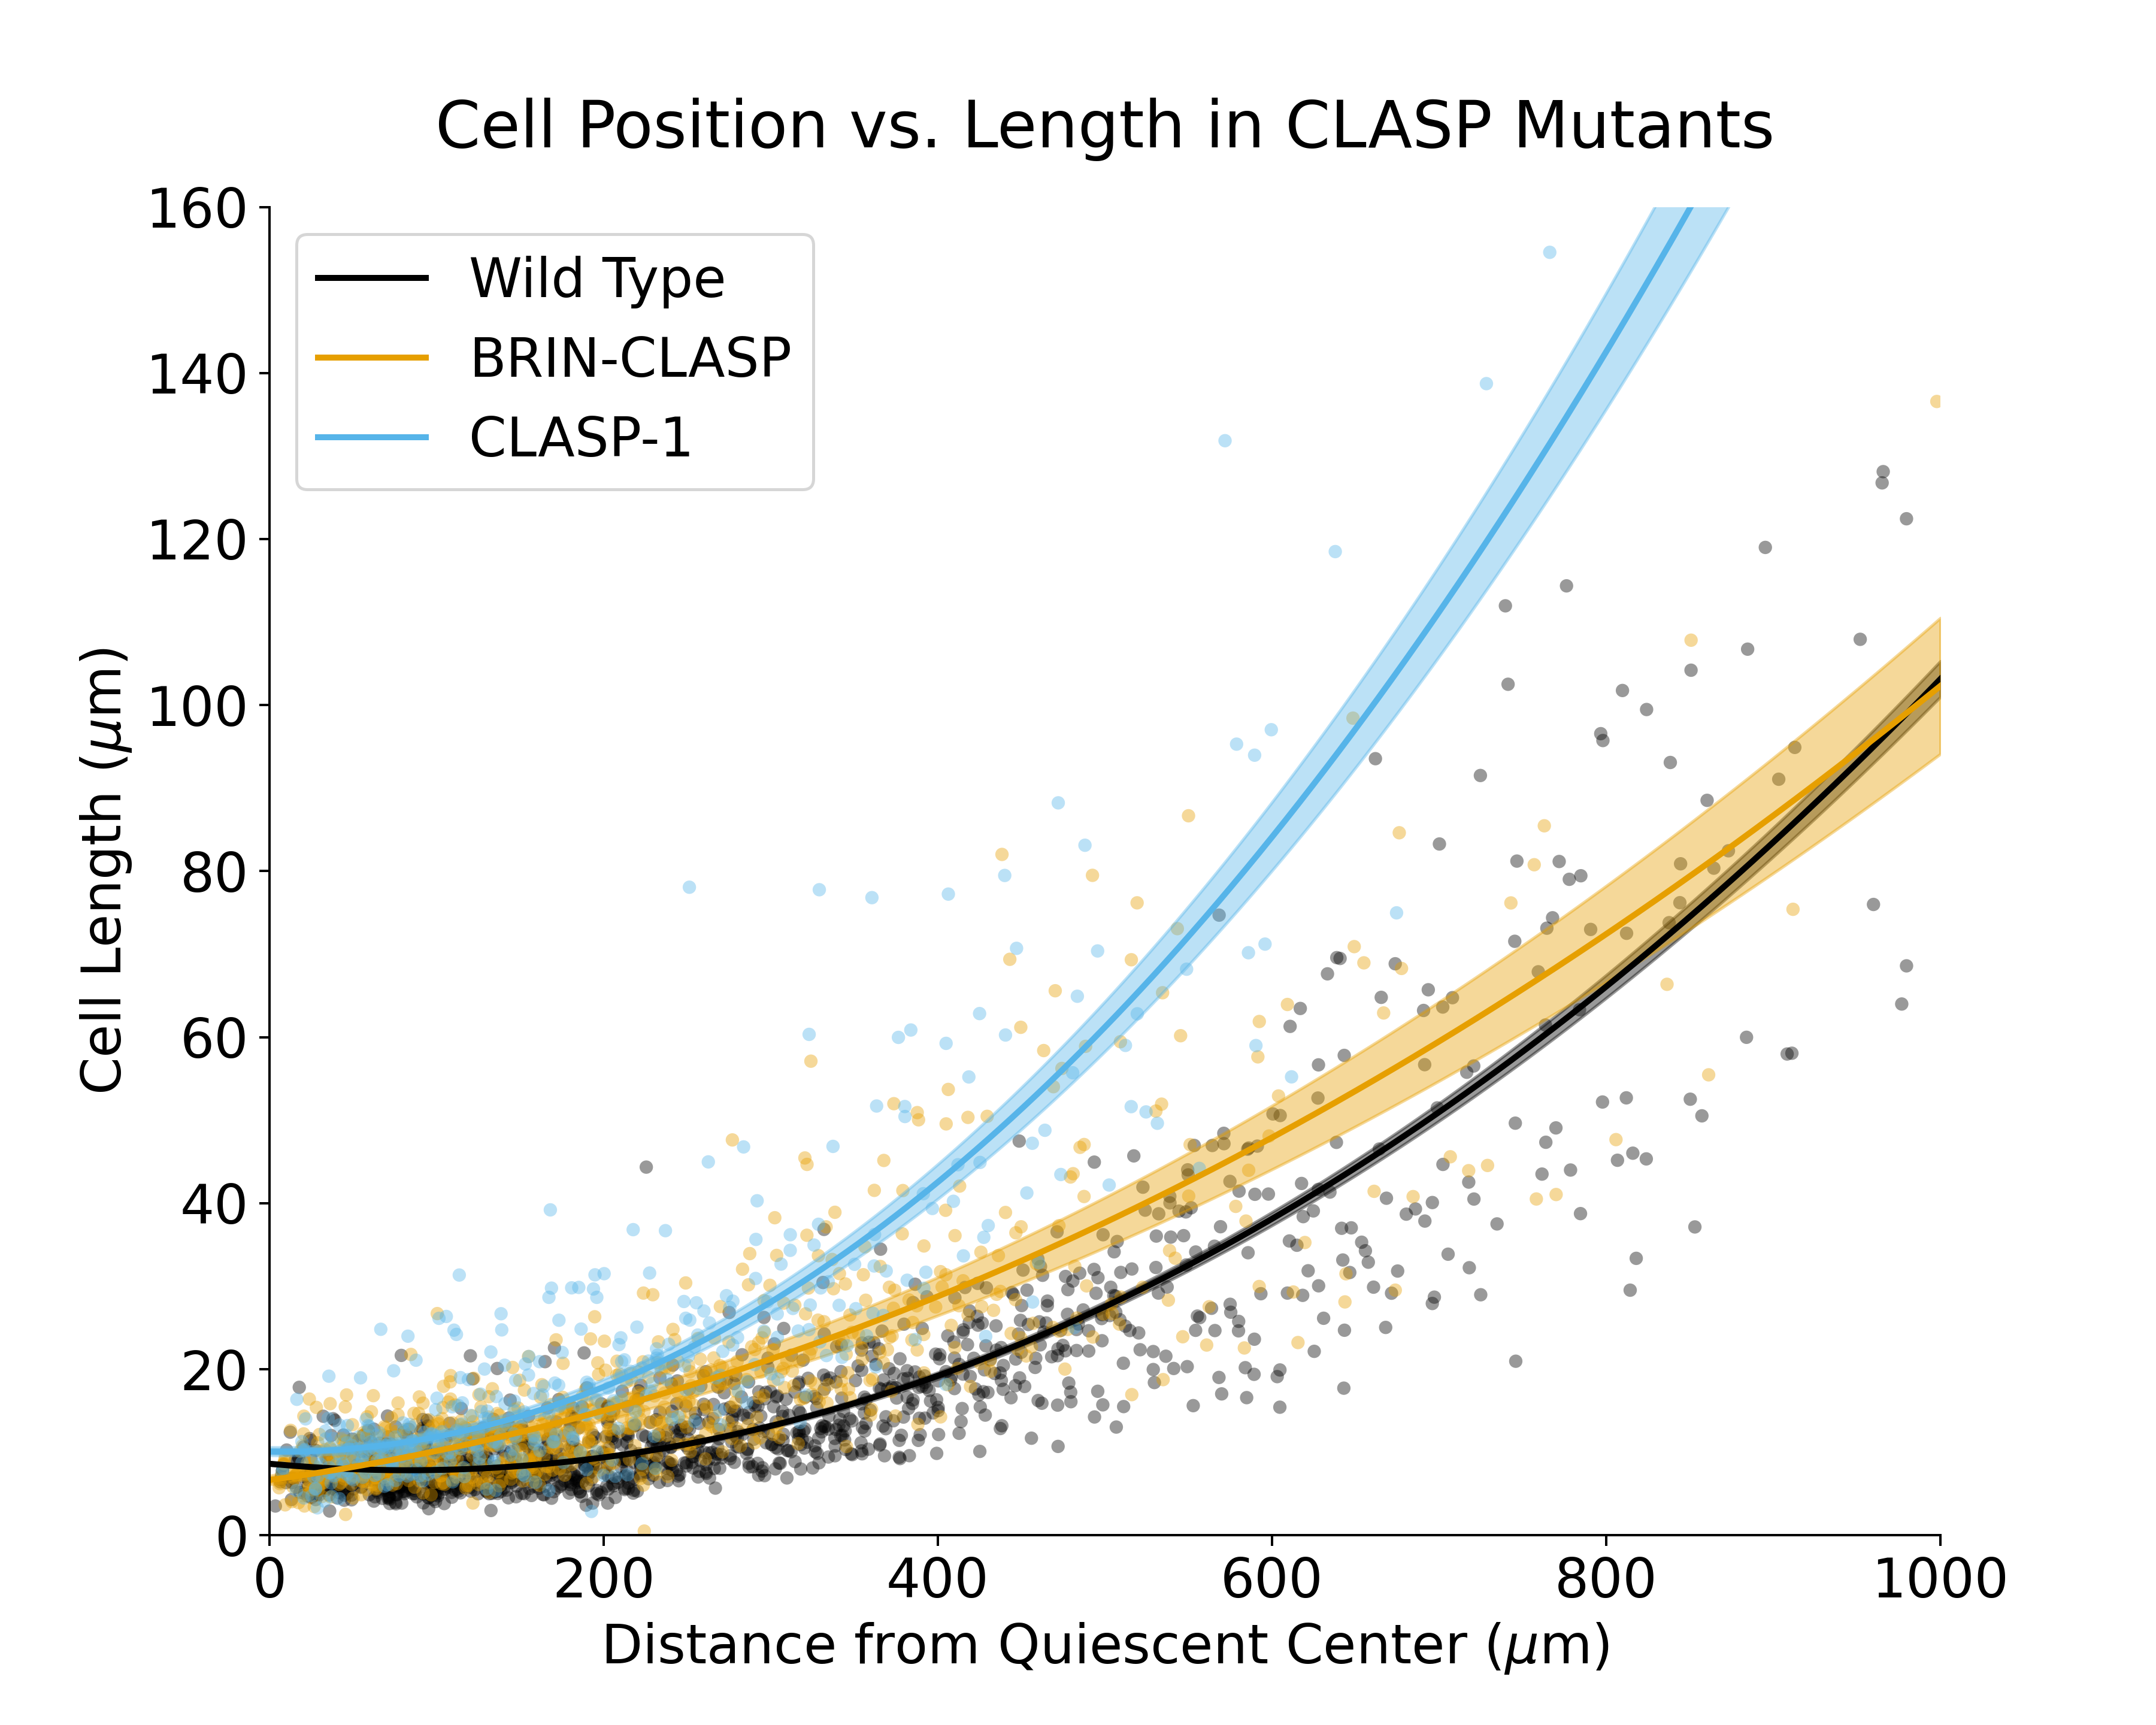
\includegraphics[width=13cm]{img/data-trichoblast.png}
    \caption{Plot of cell lengths from trichoblast cells in wild type, CLASP-1, and BRIN-CLASP roots. The line of best fit is an exponential function of the form $A + Be^{Cx}$. Wild type cells are on average the shortest, followed closely by BRIN-CLASP. CLASP-1 cells are significantly longer, especially in the proximal regions of the root. There is a large amount of variance in the data, especially at higher positions.}
    \label{sfig:data-trichoblast}
\end{supplementaryfigure}

\medskip

We wish to quantify the differences between the mutants in order to confirm that their behaviour is indeed different from the wild type. To do this, we computed the relative error of each data point from the line of best fit for the wild type cells. The distribution of these errors is shown in Figure \ref{sfig:trichoblast-distribution}. Cells in the BRIN-CLASP root have a mean error of $+41\%$ from the wild type average, while cells in the CLASP-1 root have a mean error of $+80.9\%$. This suggests a significant effect size for the various mutations. Additionally, the mutations were statistically significant with $p$-values less than $10^{-20}$, which provides further evidence that the mutants are exhibiting different behaviour.

\begin{supplementaryfigure}
    \centering
    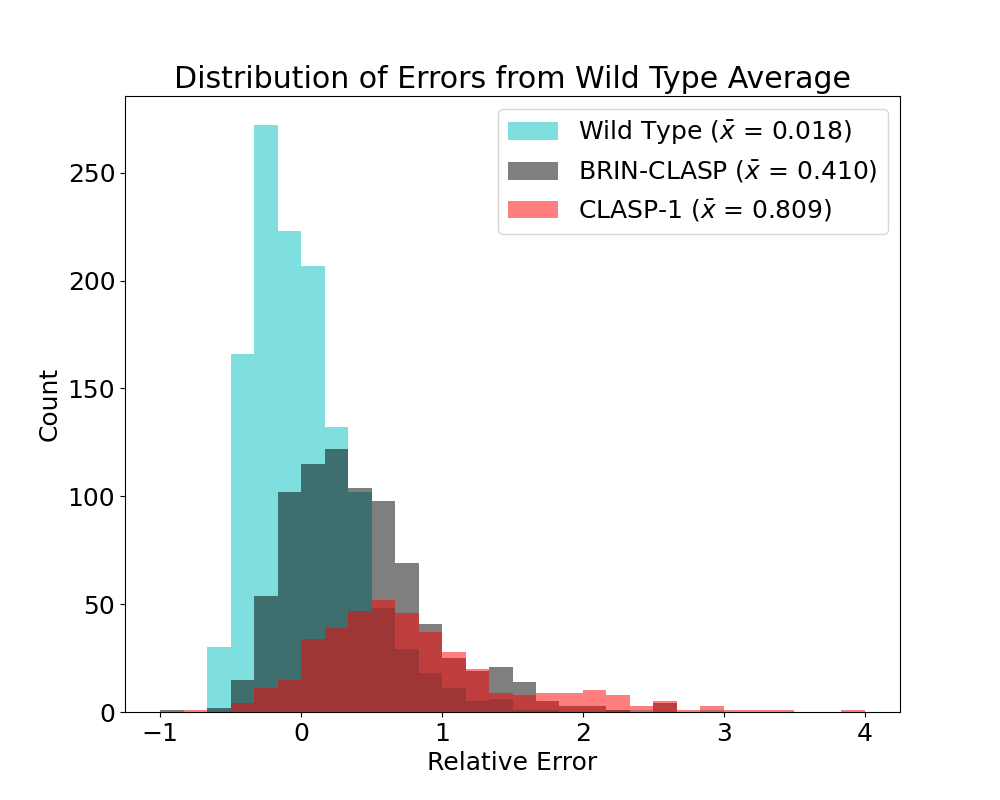
\includegraphics[width=13cm]{img/trichoblast-distribution.png}
    \caption{Distribution of errors from the wild type average presented in Figure \ref{sfig:data-trichoblast}. The mean error of the BRIN-CLASP and CLASP-1 mutants are clearly positive, which suggests that on average, the mutants have longer cells compared to the wild type. }
    \label{sfig:trichoblast-distribution}
\end{supplementaryfigure}



\subsection{Cell Column Model}

\begin{supplementaryfigure}
    \centering
    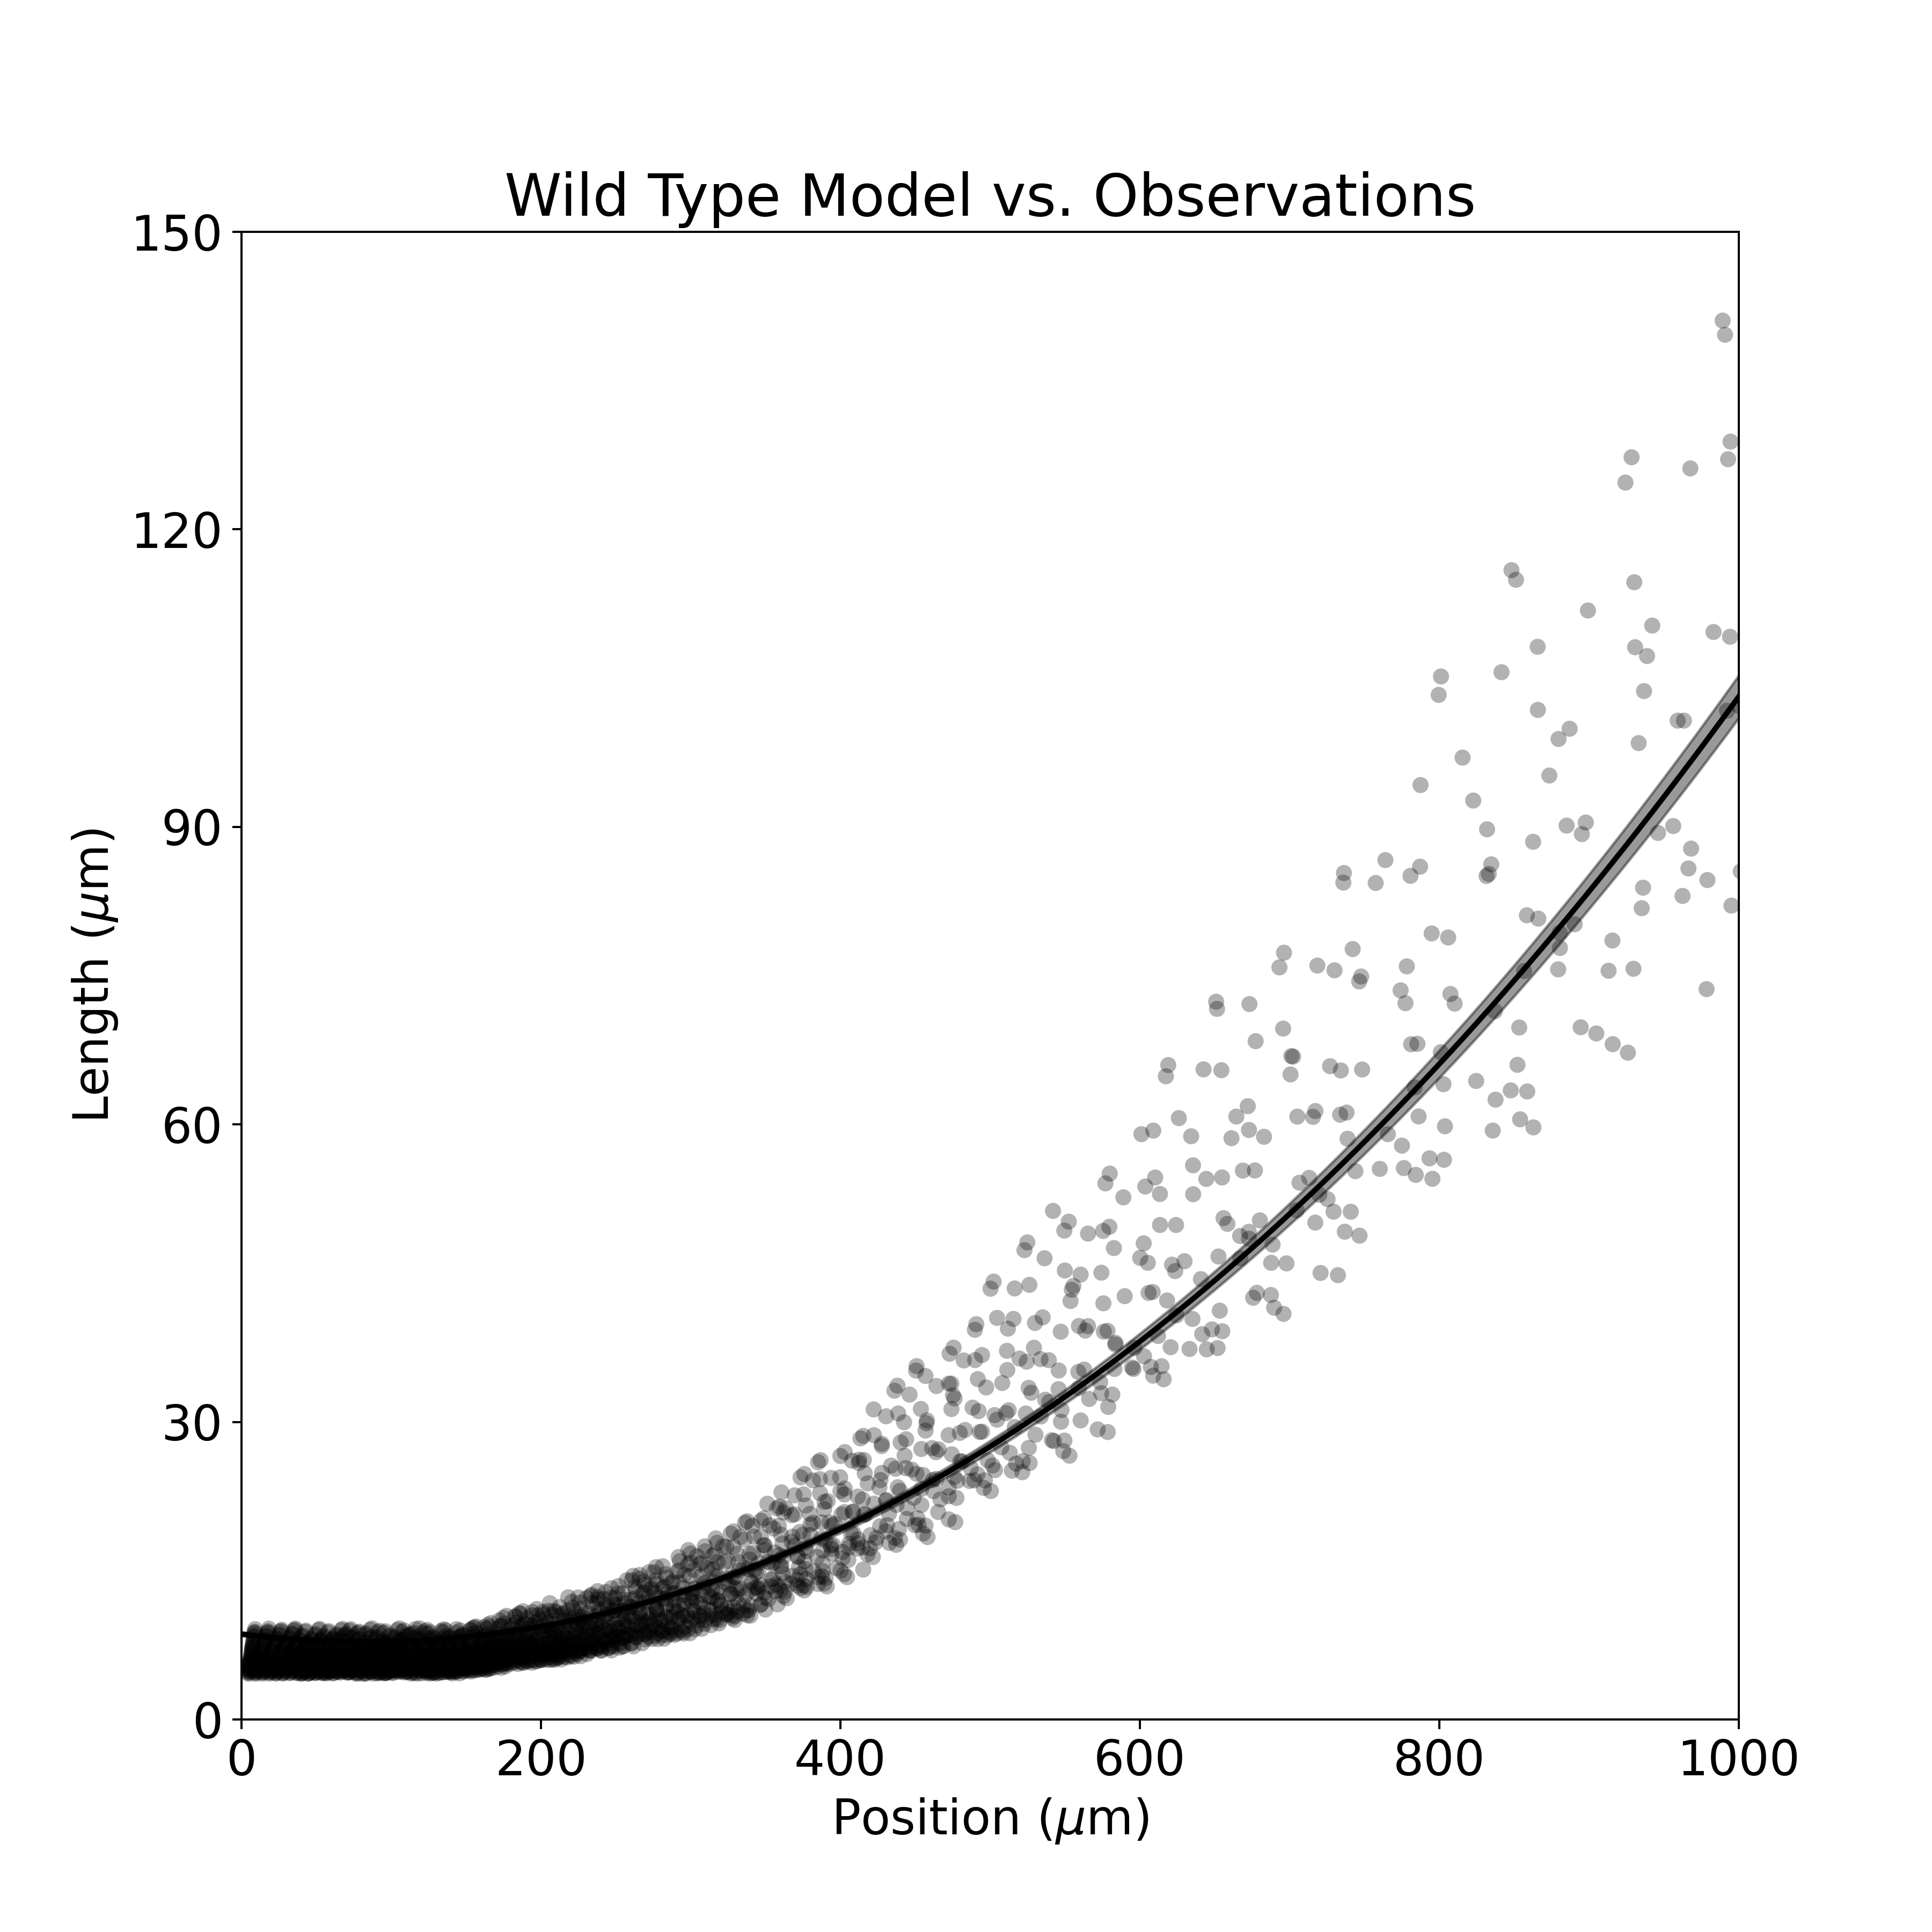
\includegraphics[width=13cm]{column-wild-type.png}
    \caption{Comparison of wild type cell column model with observations.}
    \label{sfig:column-wild-type}
\end{supplementaryfigure}

\begin{supplementaryfigure}
    \centering
    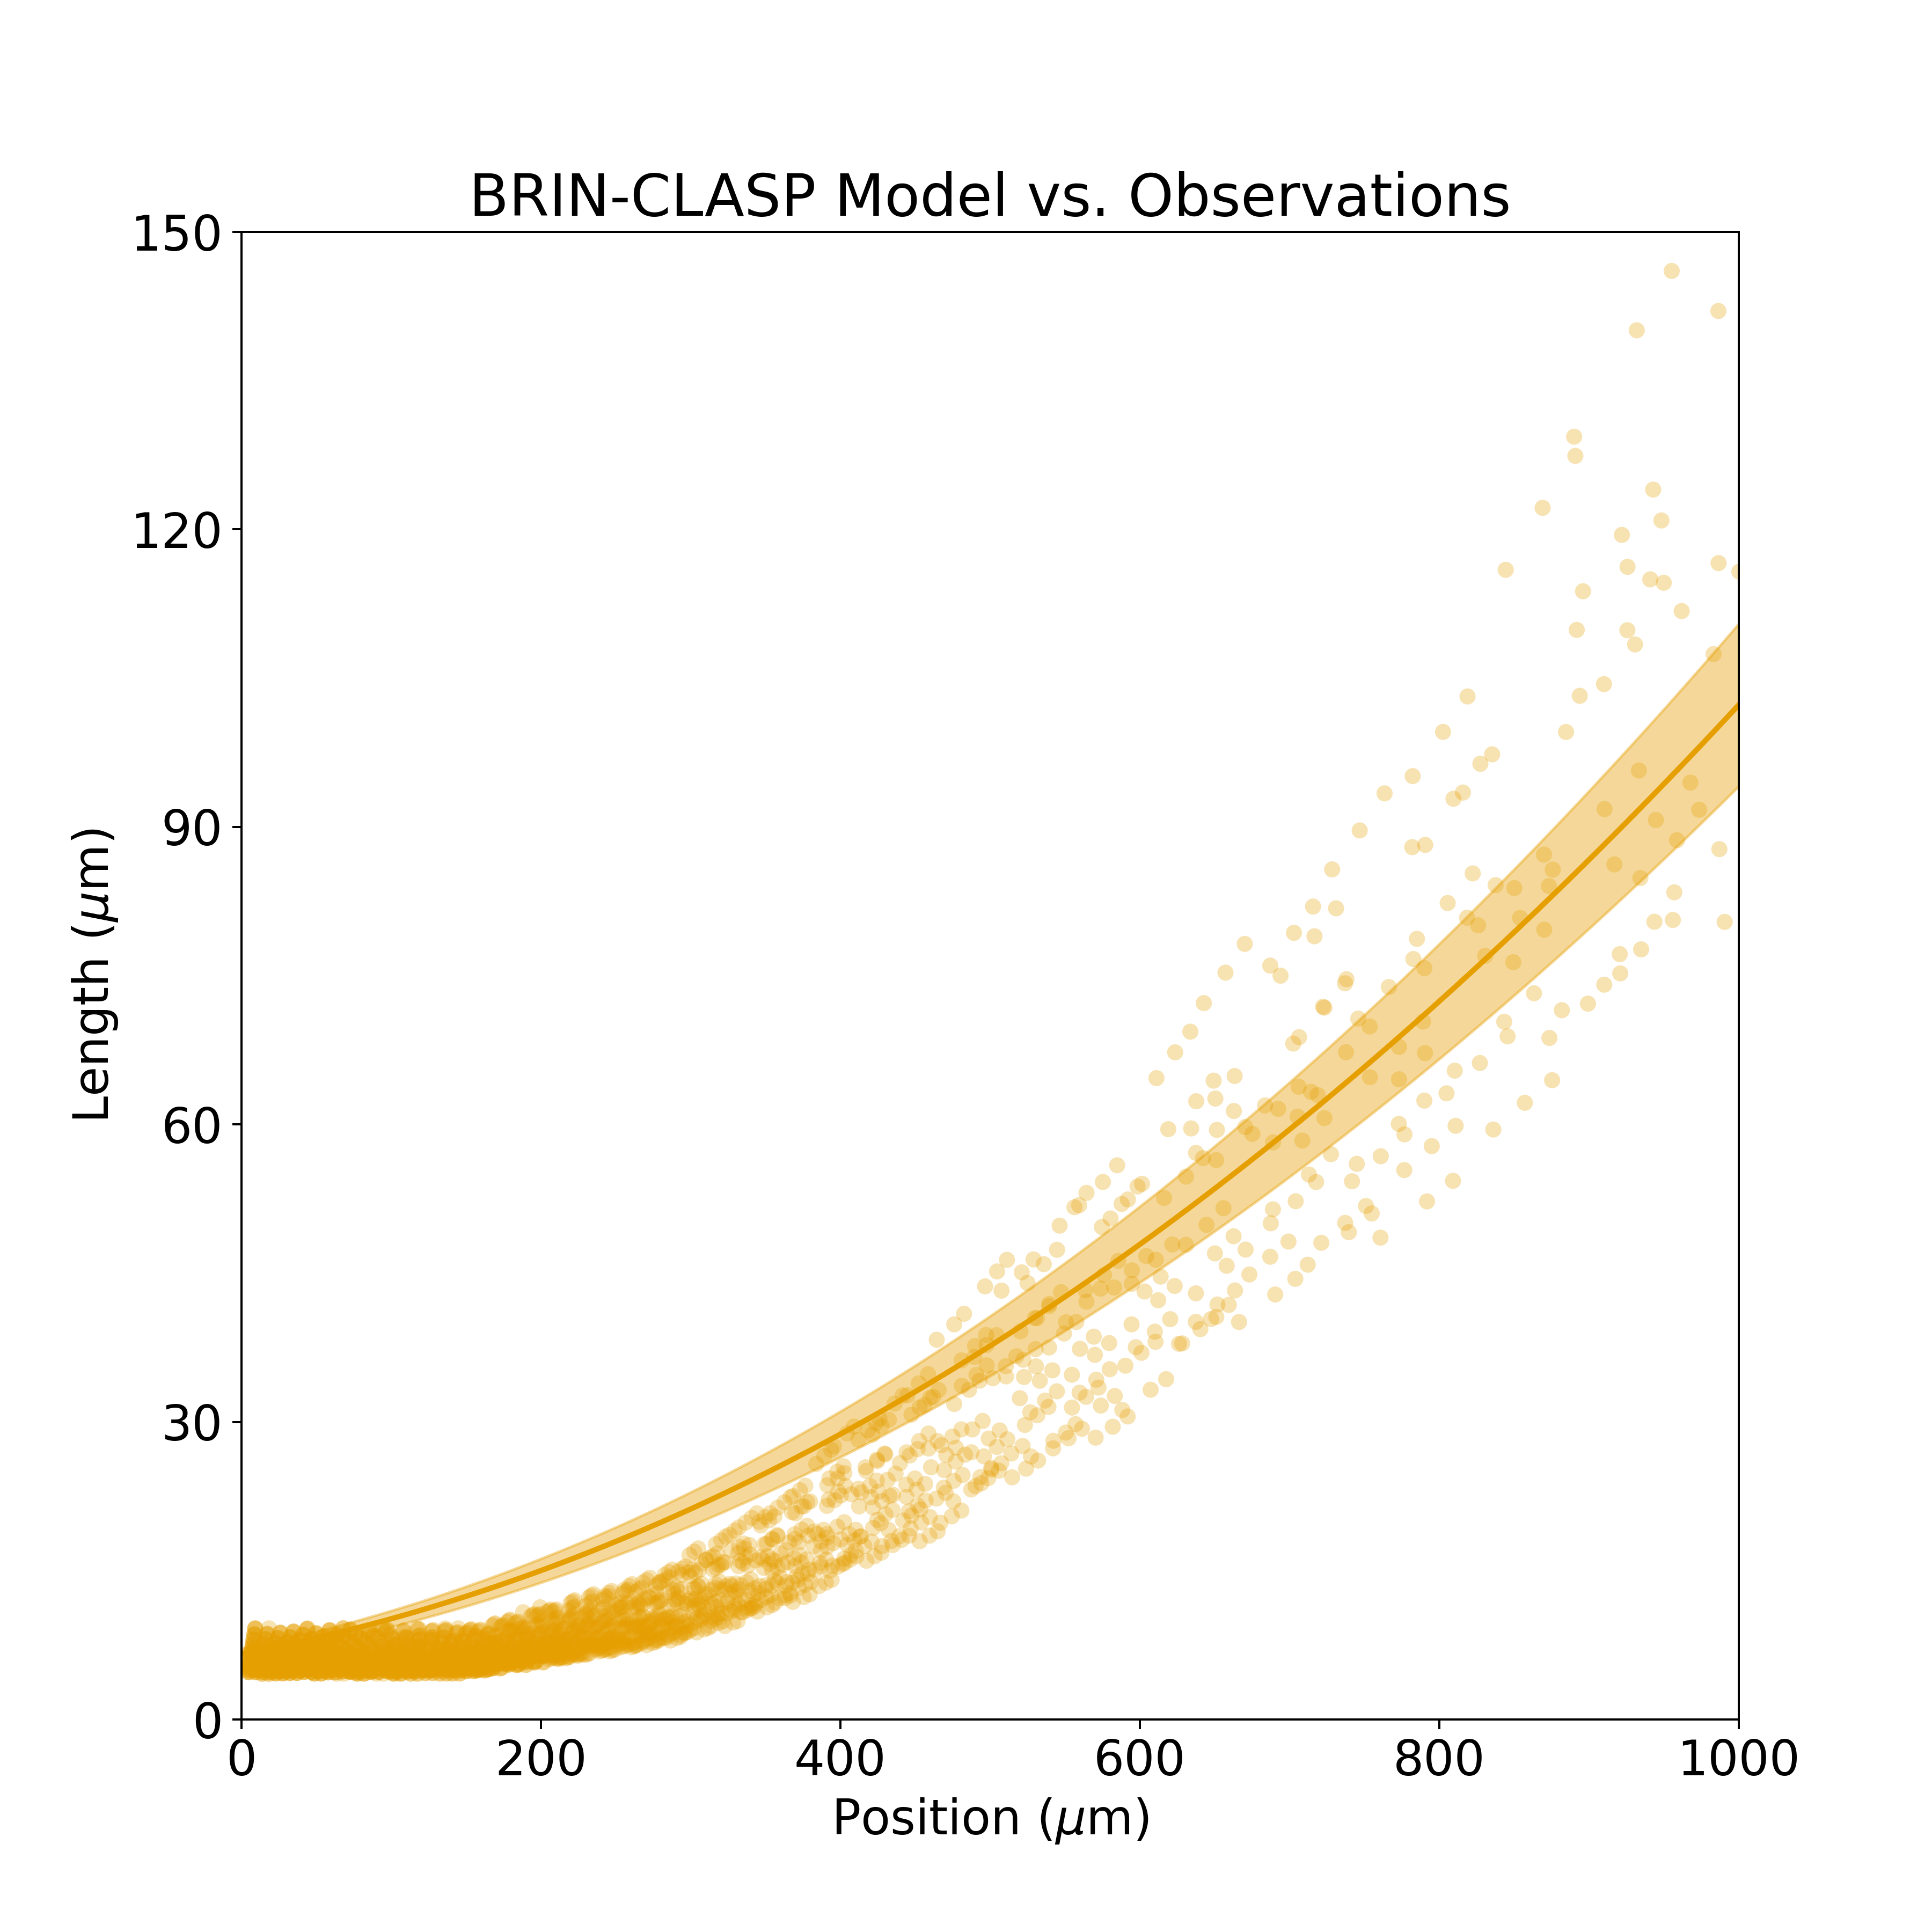
\includegraphics[width=13cm]{column-brin-clasp.png}
    \caption{Comparison of BRIN-CLASP cell column model with observations.}
    \label{sfig:column-brin-clasp}
\end{supplementaryfigure}

\begin{supplementaryfigure}
    \centering
    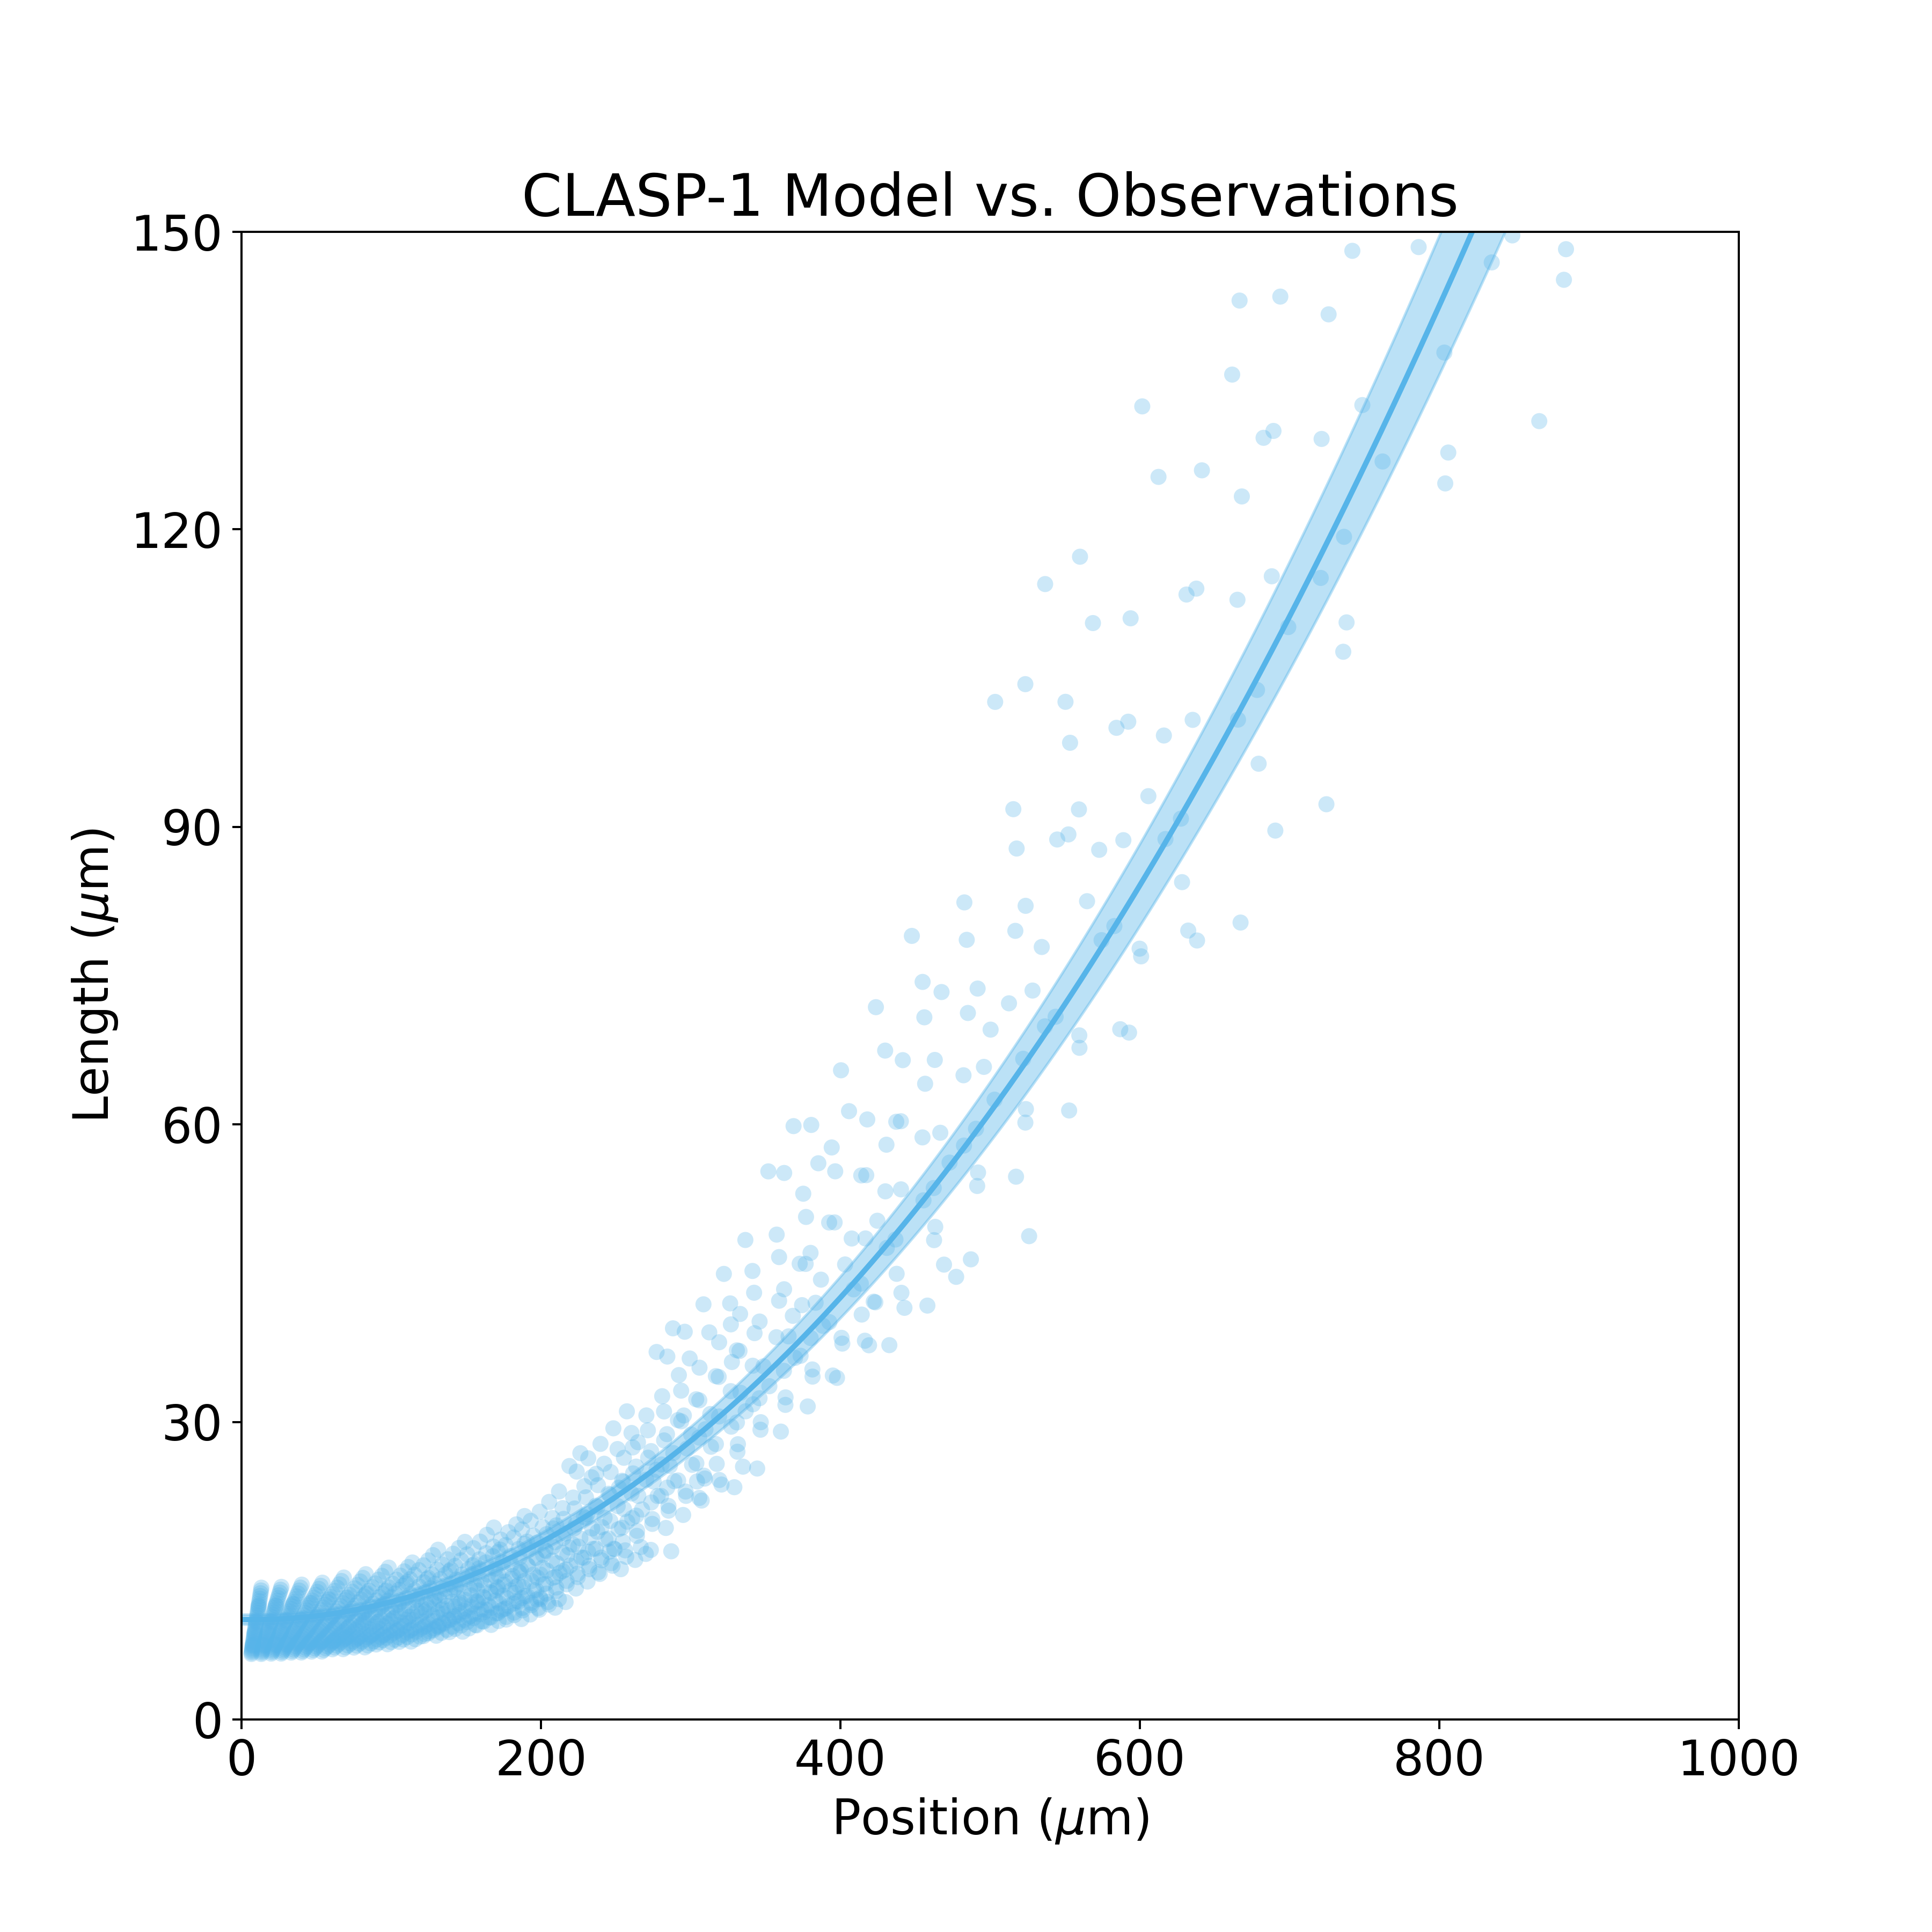
\includegraphics[width=13cm]{column-clasp-1.png}
    \caption{Comparison of CLASP-1 cell column model with observations.}
    \label{sfig:column-clasp-1}
\end{supplementaryfigure}

\begin{supplementaryfigure}
    \centering
    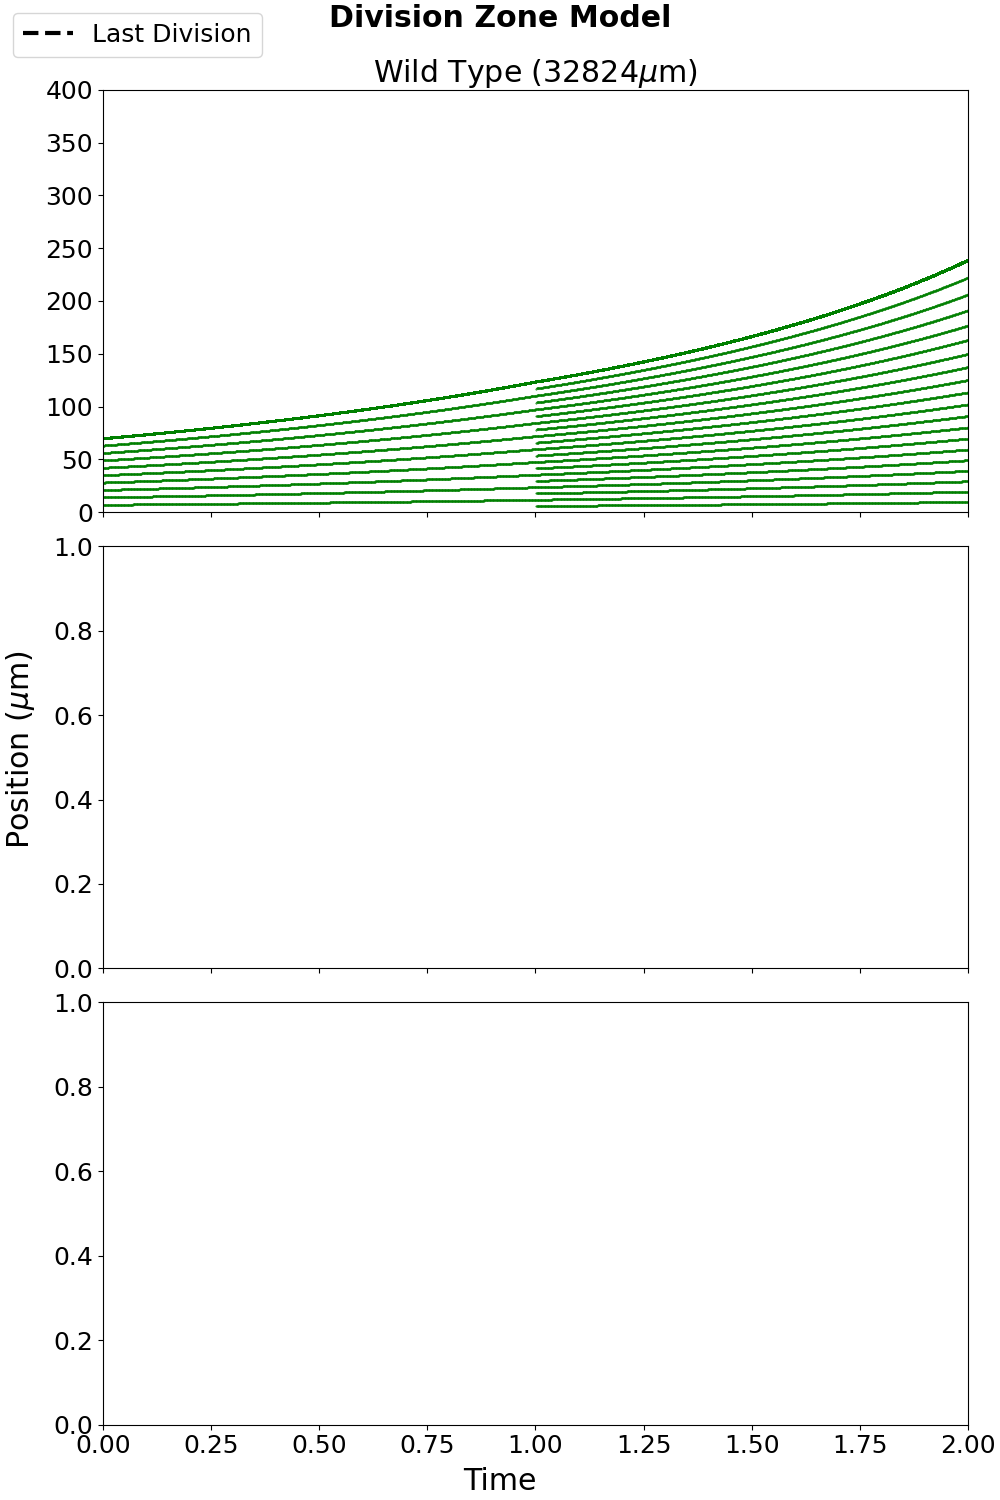
\includegraphics[width=13cm]{column-division-zone.png}
    \caption{A plot of the simulated cells in the division zone.}
    \label{sfig:column-division-zone}
\end{supplementaryfigure}

\begin{supplementaryfigure}
    \centering
    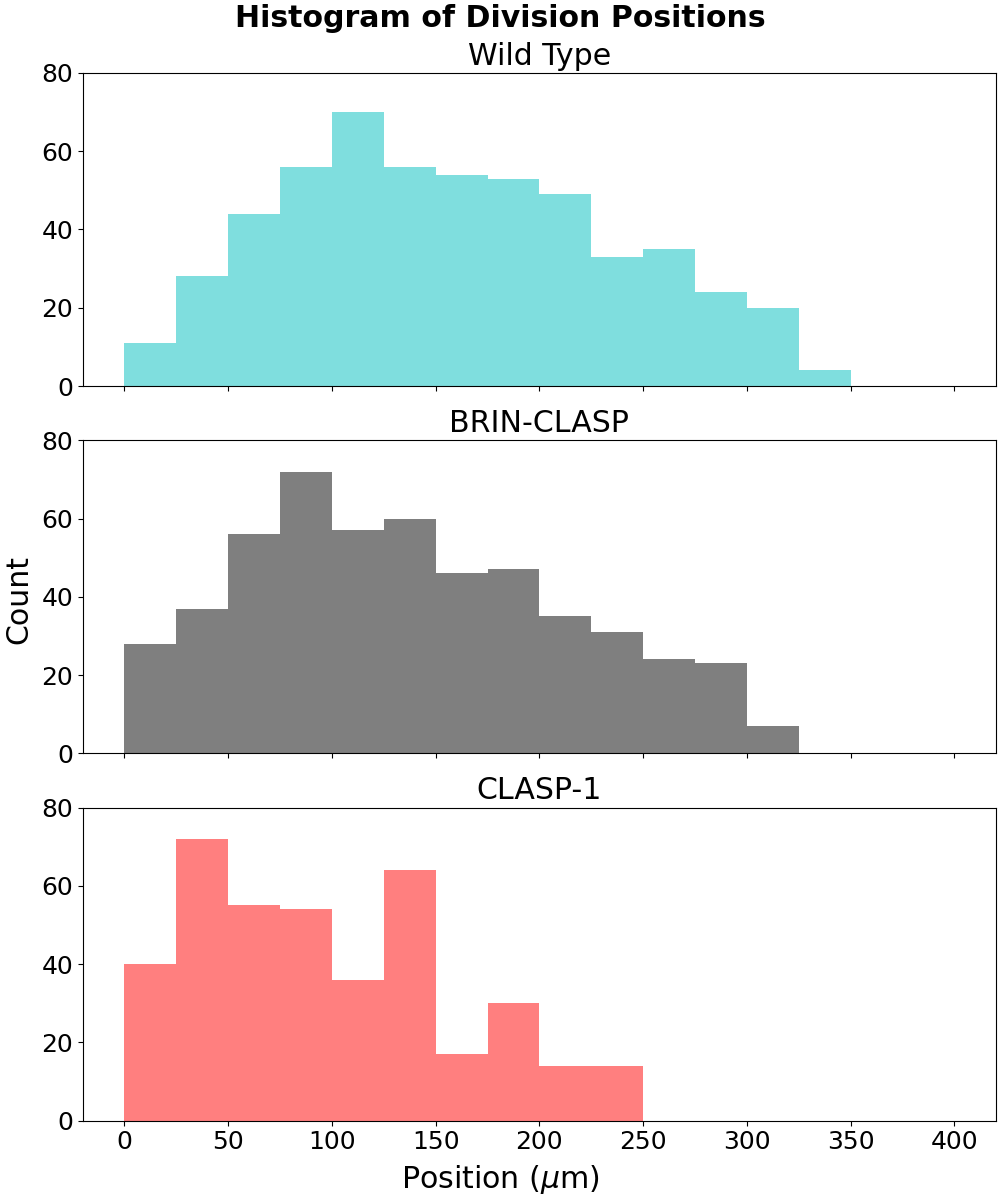
\includegraphics[width=13cm]{column-division-histogram.png}
    \caption{A histogram of division positions in each the two mutants and wild type.}
    \label{sfig:column-division-histogram}
\end{supplementaryfigure}

\subsection{Single Cell BES1 Model}

\begin{supplementaryfigure}[!htbp]
    \centering
    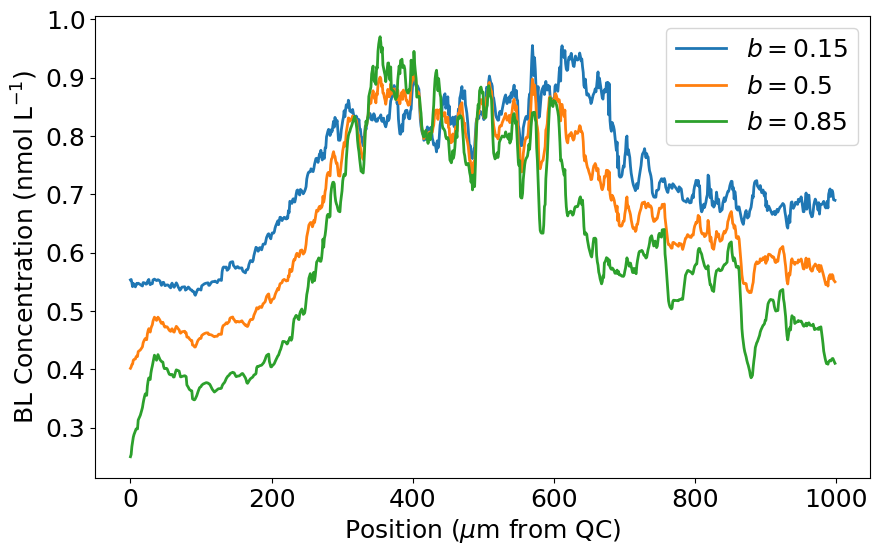
\includegraphics[width=13cm]{img/bl-bias.png}
    \caption{The BL concentration function for three different values of the bias parameter $b$. For future simulations we will use $b = 0.5$, since the BL concentration function exhibits similar qualitative behaviour for all $b$ as shown above.}
    \label{sfig:bl-bias}
\end{supplementaryfigure}

\begin{supplementaryfigure}[!htbp]
    \centering
    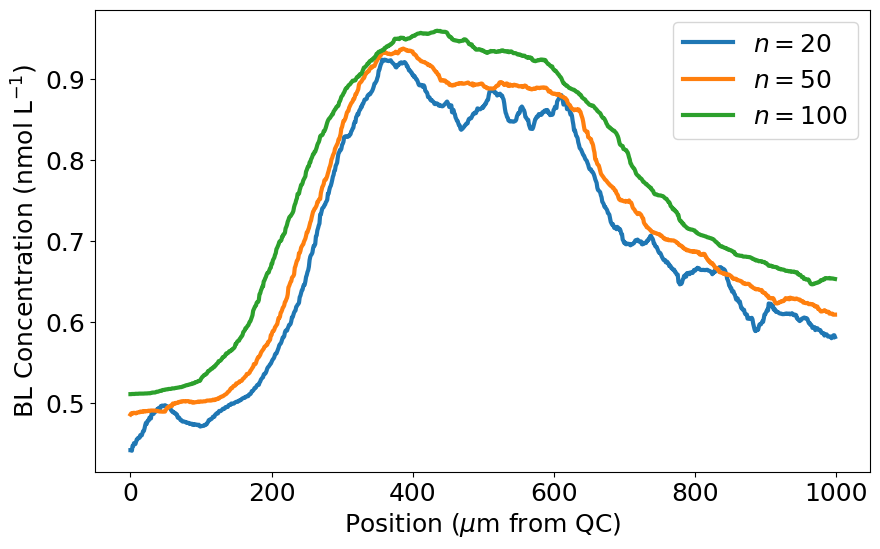
\includegraphics[width=13cm]{img/bl-average.png}
    \caption{A plot of BL concentration functions ($b = 0.5$) for three different values of the moving average period $n$. Future simulations will use $n = 50$, an admittedly arbitrary choice since the exact details of the diffusive effect we are modelling are unknown.}
    \label{sfig:bl-average}
\end{supplementaryfigure}

\begin{supplementaryfigure}
    \centering
    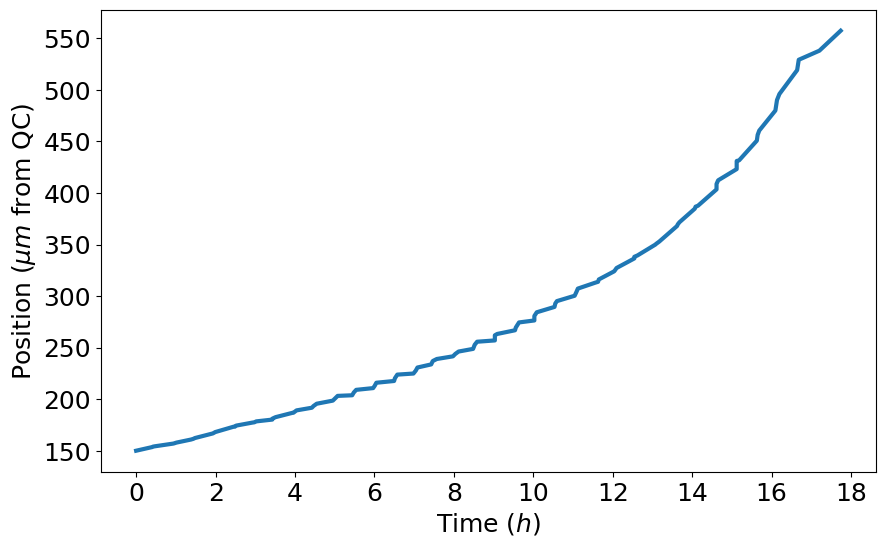
\includegraphics[width=13cm]{position-function.png}
    \caption{Plot of cell position (in $\um$) versus time (in $\h$) using cell lineage data from \cite{goh2023}. The function is scaled such that $t = 0\h$ corresponds to a position of $150\um$ above the QC.}
    \label{sfig:position-function}
\end{supplementaryfigure}

\begin{supplementaryfigure}
    \centering
    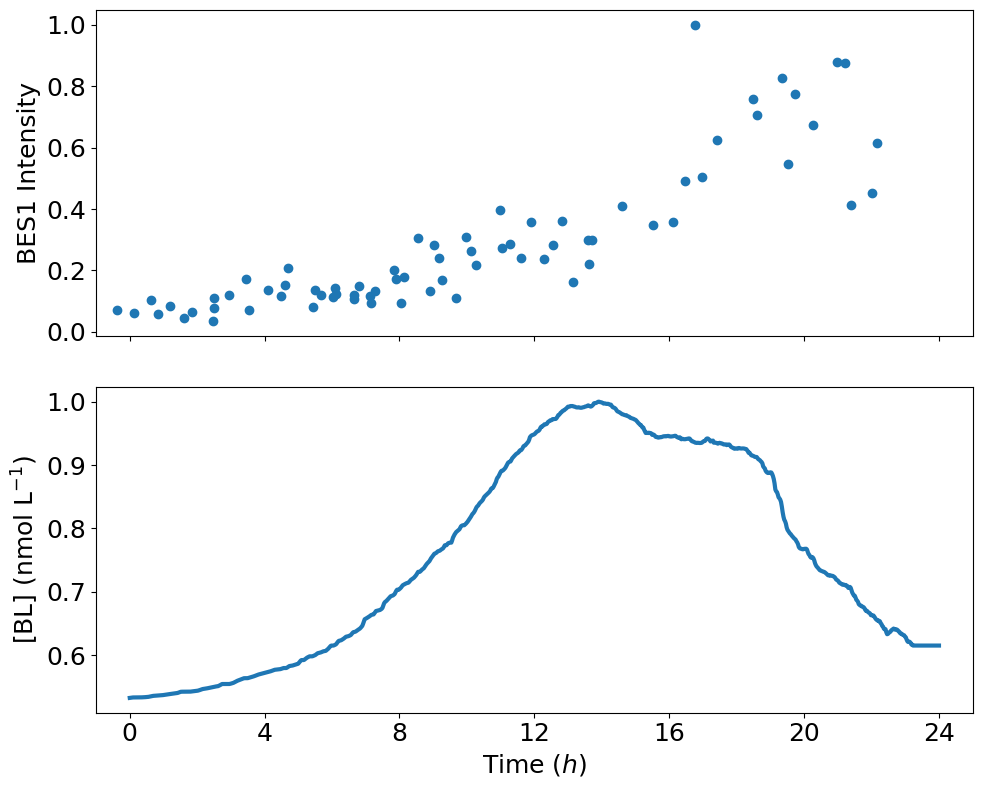
\includegraphics[width=13cm]{bes1-data.png}
    \caption{Plot of the transformed BES1 signalling data from \cite{vukasinovic2021} (left) and transformed BL concentration function (right). Since fluorescence intensity data is measured in arbitrary units, the BES1 plot was rescaled to a maximum value of $1$.}
    \label{sfig:bes1-data}
\end{supplementaryfigure}





\newpage
\printbibliography

\end{document}
